%%---------------------------------------------------------------------------%%
%% Monte Carlo Synthetic-Acceleration Paper
%% Submitted to Journal of Computational Physics 2012
%%---------------------------------------------------------------------------%%
%%
%% Copyright 2007, 2008, 2009 Elsevier Ltd
%%
%% This file is part of the 'Elsarticle Bundle'.
%% ---------------------------------------------
%%
%% It may be distributed under the conditions of the LaTeX Project Public
%% License, either version 1.2 of this license or (at your option) any
%% later version.  The latest version of this license is in
%%    http://www.latex-project.org/lppl.txt
%% and version 1.2 or later is part of all distributions of LaTeX
%% version 1999/12/01 or later.
%%
%% The list of all files belonging to the 'Elsarticle Bundle' is
%% given in the file `manifest.txt'.
%%

%%---------------------------------------------------------------------------%%
%% Document Options
%%---------------------------------------------------------------------------%%
%% Template article for Elsevier's document class `elsarticle'
%% with numbered style bibliographic references
%% SP 2008/03/01
%%
%%
%%
%% $Id: elsarticle-template-num.tex 4 2009-10-24 08:22:58Z rishi $
%%
%%
\documentclass[preprint,12pt]{elsarticle}

%% Use the option review to obtain double line spacing
%% \documentclass[preprint,review,12pt]{elsarticle}

%% Use the options 1p,twocolumn; 3p; 3p,twocolumn; 5p; or 5p,twocolumn
%% for a journal layout:
%% \documentclass[final,1p,times]{elsarticle}
%% \documentclass[final,1p,times,twocolumn]{elsarticle}
%% \documentclass[final,3p,times]{elsarticle}
%% \documentclass[final,3p,times,twocolumn]{elsarticle}
%% \documentclass[final,5p,times]{elsarticle}
%% \documentclass[final,5p,times,twocolumn]{elsarticle}

%% if you use PostScript figures in your article
%% use the graphics package for simple commands
%% \usepackage{graphics}
%% or use the graphicx package for more complicated commands
\usepackage{epsfig} \usepackage{graphicx} \usepackage{subfigure}
%% or use the.pdffig package if you prefer to use the old commands
%% \usepackage.pdffig}

%% The amssymb package provides various useful mathematical symbols
\usepackage{amssymb}
%% The amsthm package provides extended theorem environments
\usepackage{amsthm} \usepackage{amsmath} \usepackage{tmadd,tmath}
\usepackage[mathcal]{euscript} \usepackage{color}

%% The lineno packages adds line numbers. Start line numbering with
%% \begin{linenumbers}, end it with \end{linenumbers}. Or switch it on
%% for the whole article with \linenumbers after \end{frontmatter}.
%% \usepackage{lineno}

%% natbib.sty is loaded by default. However, natbib options can be
%% provided with \biboptions{...} command. Following options are
%% valid:

%%   round  -  round parentheses are used (default)
%%   square -  square brackets are used   [option]
%%   curly  -  curly braces are used      {option}
%%   angle  -  angle brackets are used    <option>
%%   semicolon  -  multiple citations separated by semi-colon
%%   colon  - same as semicolon, an earlier confusion
%%   comma  -  separated by comma
%%   numbers-  selects numerical citations
%%   super  -  numerical citations as superscripts
%%   sort   -  sorts multiple citations according to order in ref. list
%%   sort&compress   -  like sort, but also compresses numerical citations
%%   compress - compresses without sorting
%%
%% \biboptions{comma,round}

% \biboptions{}

\journal{Computational Physics}

%%---------------------------------------------------------------------------%%
%% Math Variables
%%---------------------------------------------------------------------------%%
\newcommand{\email}[1]{$\langle$#1@lanl.gov$\rangle$}

\newcommand{\vA}{\ensuremath{\ve{A}}}
\newcommand{\vb}{\ensuremath{\ve{b}}}
\newcommand{\vx}{\ensuremath{\ve{x}}}
\newcommand{\vr}{\ensuremath{\ve{r}}}
\newcommand{\vu}{\ensuremath{\ve{u}}}
\newcommand{\vI}{\ensuremath{\ve{I}}}
\newcommand{\vH}{\ensuremath{\ve{H}}}
\newcommand{\vP}{\ensuremath{\ve{P}}}

\newcommand{\Cv}{\ensuremath{C_{v}}}
\newcommand{\ros}{\ensuremath{\sigma_{\scriptscriptstyle\mathrm{R}}}}
\newcommand{\bOmega}{\ensuremath{\mathbf{\Omega}}}

\newcommand{\dt}{\ensuremath{\Delta t}}
\newcommand{\sign}{\ensuremath{\tilde{\sigma}^n}}
\newcommand{\qn}{\ensuremath{q^n}} \newcommand{\Tn}{\ensuremath{T^n}}
\newcommand{\Dn}{\ensuremath{D^n}}
\newcommand{\phin}{\ensuremath{\phi^n}}
\newcommand{\Di}{\ensuremath{\Delta_i}}
\newcommand{\Dj}{\ensuremath{\Delta_j}}
\newcommand{\Dk}{\ensuremath{\Delta_k}}

\newcommand{\sigT}{\ensuremath{\sigma_{T\,ijk}}}
\newcommand{\sigm}{\ensuremath{\sigma^{-}}}
\newcommand{\sigp}{\ensuremath{\sigma^{+}}}

\newcommand{\bphi}{\ensuremath{\boldsymbol{\phi}}}

\DeclareMathOperator{\diag}{diag}

%%---------------------------------------------------------------------------%%
\begin{document}

\begin{frontmatter}

  \title{A Monte Carlo Synthetic-Acceleration Method for Solving the Thermal
    Radiation Diffusion Equation\tnoteref{ornl-cr}}
  \tnotetext[ornl-cr]{Notice: This manuscript has been authored by
    UT-Battelle, LLC, under contract DE-AC05-00OR22725 with the
    U.S. Department of Energy. The United States Government retains and the
    publisher, by accepting the article for publication, acknowledges that the
    United States Government retains a non-exclusive, paid-up, irrevocable,
    world-wide license to publish or reproduce the published form of this
    manuscript, or allow others to do so, for United States Government
    purposes.}

  \author[ornl]{Thomas M. Evans\corref{cor1}\fnref{fn1}} \ead{evanstm@ornlgov}
  \cortext[cor1]{Corresponding Author}

  \author[ornl]{Scott W. Mosher\fnref{fn1}} \ead{moshersw@ornl.gov}

  \author[wisc]{Stuart R. Slattery\fnref{fn2}} \ead{sslattery@wisc.edu}

  \fntext[fn1]{Radiation Transport Group, Reactor and Nuclear Systems
    Division} \fntext[fn2]{Department of Engineering Physics, College of
    Engineering}

  \address[ornl]{Oak Ridge National Laboratory, 1 Bethel Valley Rd., Oak
    Ridge, TN 37831 U.S.A.}  \address[wisc]{University of Wisconsin-Madison,
    1500 Engineering Dr., Madison, WI 53716 U.S.A.}

  \begin{abstract}

    We present a novel synthetic-acceleration-based Monte Carlo method for
    solving the equilibrium thermal radiation diffusion equation in three
    spatial dimensions. The algorithm performance is compared against
    traditional solution techniques using a Marshak benchmark problem and a
    more complex multiple material problem. Our results show that our Monte
    Carlo method is an effective solver for sparse matrix systems. For
    solutions converged to the same tolerance, it performs competitively with
    deterministic methods including preconditioned conjugate gradient. We also
    discuss various aspects of preconditioning the method and its general
    applicability to broader classes of problems.

  \end{abstract}

  \begin{keyword}
    radiation diffusion \sep synthetic acceleration \sep Monte Carlo
    \sep sparse matrix systems
  \end{keyword}

\end{frontmatter}

%% main text
%%---------------------------------------------------------------------------%%
\section{Introduction}
\label{sec:introduction}

In previous work~\cite{evans_2003}, we developed a residual Monte Carlo method
that was an application of Halton's Sequential Monte Carlo
method~\cite{halton_1962,halton_1994} to the one-dimensional (1D) equilibrium
thermal radiation diffusion equation.  At that time, Halton's method was not
widely known in the general computational physics community.  While extending
our method to three spatial dimensions, we realized that the Sequential Monte
Carlo method is actually a variant of iterative refinement cast as a residual
method. We have developed a new method in which Monte Carlo is used to
accelerate a fixed-point (Richardson) iteration. This algorithm surpasses our
previous 1D method and allows for extension to more general solution
techniques.

The purpose of this study is to demonstrate an efficient Monte Carlo solution
method for three-dimensional (3D), time-dependent, discrete systems. In this
work, our previous investigations are extended in the following manner:
\begin{itemize}
\item we develop a rigorous synthetic-acceleration Monte Carlo method
  for solving sparse matrix systems;
\item we apply this method to the one-temperature (1T) thermal radiation
  diffusion equation in three dimensions;
\item we compare numerical and performance results of the Monte Carlo
  method against traditional deterministic solution methods.
\end{itemize}

In \S~\ref{sec:monte-carlo-matrix} we review Monte Carlo methods for solving
matrix systems, and we discuss our new synthetic-acceleration scheme and
connect it with previous work by Halton~\cite{halton_1994} and
others~\cite{evans_2003}.  The 1T radiation diffusion equation and its
discrete form will be derived in \S~\ref{sec:discr-form-radi}.  We discuss
using Monte Carlo Synthetic-Acceleration to solve the discrete radiation
diffusion equation in \S~\ref{sec:solut-radi-diff}.  Results from two 3D test
problems are given in \S~\ref{sec:results}.  We finish with conclusions and
ideas for future work in \S~\ref{sec:conclusions}.

%%---------------------------------------------------------------------------%%
\section{Mathematical Methods}
\label{sec:monte-carlo-matrix}

The idea of using Monte Carlo methods (random walks) to invert linear systems
is not new.  The earliest referenced work dates to a 1950 paper by Forsythe
and Leibler \cite{forsythe}.  Their paper credits the idea to unpublished work
by J.v. Neumann and S.M. Ulam dating back to the 1940's.  The basic principles
of Monte Carlo matrix inversion were further elucidated in Hammersley and
Handscomb's 1964 text \cite{hammersley_1964}.  These early methods are
distinguished by very slow, statistically noisy convergence properties; thus,
they have not made any significant impact in the physics community.

In order to address the convergence issues plaguing Monte Carlo
solvers, Halton \cite{halton_1962,halton_1994} proposed a Sequential
Monte Carlo method.  This algorithm demonstrated dramatically improved
convergence over regular Monte Carlo.  Nonetheless, Halton's method
has not gained widespread use in computational physics
applications. In the next sections, we will briefly describe the Monte
Carlo methods that can be used to solve linear systems and expand them
to present our new synthetic-acceleration method.

%%---------------------------------------------------------------------------%%
\subsection{Monte Carlo Matrix Solution Methods}
\label{sec:background}

To establish the mathematical framework for Monte Carlo linear
solvers, we consider the following matrix equation:
\begin{equation}
  \vA\vx = \vb\:,
  \label{eq:Ax=b}
\end{equation}
which can be written as
\begin{equation}
  \begin{split}
    \vx &= (\vI - \vA)\vx + \vb\\ &= \vH\vx + \vb\:.
  \end{split}
  \label{eq:point_iteration}
\end{equation}
When the spectral radius ($\rho$) of the iteration matrix ($\vH$) is
less than 1, we can expand $\vA^{-1}$ using the \latin{Neumann
  Series}:
\begin{equation}
  \vA^{-1} = (\vI - \vH)^{-1} = \sum_{k=0}^{\infty} \vH^k\:.
\end{equation} 
Thus, when $\rho(\vH) < 1$, we can recast the solution vector $\vx$ as
a series:
\begin{equation}
  \begin{split}
    \vx &= (\vI - \vH)^{-1}\vb\\ &= \vb + \vH\vb + \vH^2\vb + \vH^3\vb
    + \ldots\:.
    \label{eq:neumann_series}
  \end{split}
\end{equation}
With this knowledge in hand, we can write an iterative method that
solves Eq.~(\ref{eq:Ax=b}) (Richardson's Iteration):
\begin{equation}
  \vx^{k+1} = \vH\vx^k + \vb\:.
  \label{eq:richardson}
\end{equation}
Equation~(\ref{eq:richardson}) will converge for all $\vb,\vx^0 \in
\mathcal{R}^{N}$ when $\rho(\vH) < 1$~\cite{kelley_1995}.  All of the Monte
Carlo methods that are described in \S\S~\ref{sec:direct-method} through
\ref{sec:iter-refin-monte} rely on estimating the terms in
Eq.~(\ref{eq:neumann_series}) through random walks.

%%---------------------------------------------------------------------------%%
\subsubsection{Direct Method}
\label{sec:direct-method}

Now we consider a Monte Carlo method that can be used to estimate the
solution to Eq.~(\ref{eq:Ax=b})~\cite{hammersley_1964}.  First,
rewrite Eq.~(\ref{eq:neumann_series}) in order to calculate a
component of $\vx$:
\begin{equation}
  \begin{split}
    x_i &= (\vb)_i + (\vH\vb)_i + (\vH^2\vb)_i + (\vH^3\vb)_i +
    \ldots\\ &= \sum_{k=0}^{\infty}\sum_{i_1}^{N}\sum_{i_2}^{N}\ldots
    \sum_{i_k}^{N}h_{i,i_1}h_{i_1,i_2}\ldots h_{i_{k-1},i_k}b_{i_k}\:.
  \end{split}
  \label{eq:neumann_series_i}
\end{equation}
The terms in the Neumann series can be interpreted as a series of
transitions from $i_{m-1}\rightarrow i_m$ that can be simulated by a
random walk.  Let $X$ be a random variable sampled from a random walk
with $k$ events that initiates in state $i$:
\begin{equation}
  \begin{split}
    X(i_0 = i) &= \sum_{m=0}^{k}W_m b_{i_m}\\ &=
    \sum_{m=0}^{k}w_{i,i_1}w_{i_1,i_2}\ldots w_{i_{m-1},i_m}b_{i_m}\:.
  \end{split}
  \label{eq:estimator_xi}
\end{equation}
Here, the weight on the $m^\text{th}$ step is denoted $W_m$, and each
random walk starts with unit weight. At every step, contributions to
each component of $X$ are generated only in the starting state of the
history, $i_0$, by the source term in the current state,
$b_{i_m}$. Therefore, for a given random walk permutation, each state
must be used as a starting value in order to calculate its component
of the expectation value (i.e. a state of size $N$ will have $N$
histories per random walk permutation). When there is a transition
between states, for example $i\rightarrow j$, the weight is multiplied
by the transition factor
\begin{equation}
  w_{ij} = \frac{h_{ij}}{p_{ij}}\:,
  \label{eq:weight}
\end{equation}
where $p_{ij}$ denotes the probability of transitioning from state $i$
to $j$. Then, the expected value of $X$ is
\begin{equation}
  \begin{split}
    E[X(i_0=i)] &= \sum_{\nu}P_\nu X_\nu\\ &=
    \sum_{k=0}^{\infty}\sum_{i_1}^{N}\sum_{i_2}^{N}\ldots
    \sum_{i_k}^{N}p_{i,i_1}p_{i_1,i_2}\ldots p_{i_{k-1},i_k}
    w_{i,i_1}w_{i_1,i_2}\dots w_{i_{k-1},i_k}b_{i_k}\\ &= x_i\:,
  \end{split}
  \label{eq:expectation_xi}
\end{equation}
where $\nu$ denotes a particular random walk permutation.  Therefore,
the estimator in Eq.~(\ref{eq:estimator_xi}) is an unbiased estimator
of the components of $\vx$ provided $\rho(\vH) < 1$.

We are left to define the transition probabilities. The most
straightforward approach is to set
\begin{equation}
  p_{ij} = \frac{|h_{ij}|}{\sum_{j}|h_{ij}|}\:.
  \label{eq:probability}
\end{equation}
Each row of the transition probability matrix, $\vP$, represents a
discrete probability density function that can be sampled to select a
new state $j$, given that the current state is $i$.  Random walks can
be terminated in two ways: the matrix can be augmented with a
terminating event equation that describes the probability that a
history ends its walk, or the random walk can be terminated by weight
cutoff, $W_c$.  Generally, we choose to terminate random walks using a
weight cutoff as opposed to augmenting the matrix such that the random
walk terminates when $W_m < W_c$.

%%---------------------------------------------------------------------------%%
\subsubsection{Adjoint Method}
\label{sec:adjoint-method}

An alternative approach to the one just described is to calculate
contributions to every component of $\vx$ during the random walk. In
this method, the weight change from state $i\rightarrow j$ is
\begin{equation}
  w_{ij} = \frac{h_{ji}}{p_{ij}}\:.
  \label{eq:adjoint-weight}
\end{equation}
The transition probabilities may be calculated as
\begin{equation}
  p_{ij} = \frac{|h_{ji}|}{\sum_{j}|h_{ji}|}\:.
  \label{eq:adjoint-probability}
\end{equation}
Note that the indices are reversed so that the probabilities are normalized
over a column, as opposed to the forward method in which the probabilities are
normalized over a row.  This is equivalent to forming the Neumann series in
reverse order.  Correspondingly, the estimator for this method is
\begin{equation}
  \begin{split}
    X &= \sum_{m=0}^{k}W_m\delta_{i_m,i}\\ &=
    \sum_{m=0}^{k}\hat{b}_{i_0}w_{i_0,i_1}w_{i_1,i_2}\ldots
    w_{i_{m-1},i_m}\delta_{i_m,i}\:.
  \end{split}
  \label{eq:adjoint-tally}
\end{equation}
Here, $\hat{b}_{i_0}$ is the sampled source and initial weight in state $i_0$.
The Kronecker delta implies that tallies are only made in the state where the
random walk currently resides.  This is the common approach in standard Monte
Carlo transport simulations. Unlike the direct method, because tallies are
made in the state in which the random walk currently resides, we are no longer
required to start a history in each state for each random walk
permutation. Instead, sampling the source is sufficient and requires only one
random walk per permutation.

Similar to the direct method, the adjoint method random walk process
requires a terminating condition.  In all of the work that follows we
utilize a relative weight cutoff.  The relative weight cutoff is
defined as a fraction of the starting weight such that
\begin{equation}
  W_f = W_c\hat{b}_{i_0}\:,
  \label{eq:weight_cutoff}
\end{equation}
where $W_f$ is the terminating weight of the random walk and $W_c$ is
the input relative weight cutoff. The random walk terminates on the
$m^\text{th}$ step if $W_m < W_f$.

%%---------------------------------------------------------------------------%%
\subsection{Monte Carlo Synthetic Acceleration}
\label{sec:iter-refin-monte}

The methods presented in \S~\ref{sec:background} are characterized by slow
convergence rates bound by the Central Limit Theorem.
Halton~\cite{halton_1962,halton_1994} proposed a staged residual scheme called
Sequential Monte Carlo to speed up the convergence of these methods.  A
variant of this scheme has been successfully applied to the 1D nonlinear
thermal radiation diffusion equation in Ref.~\cite{evans_2003}.

Concisely, the Sequential Monte Carlo method solves Eq.~(\ref{eq:Ax=b}) using
the adjoint solution technique described in \S~\ref{sec:adjoint-method}.  The
following iteration scheme is applied:
\begin{subequations}
  \begin{gather}
    \vr^{l} = \vb - \vA\vx^{l}\:, \\ \vA\delta\vx^{l+1} =
    \vr^{l}\:, \label{eq:residual_solve}\\ \vx^{l+1} = \vx^{l} +
    \delta\vx^{l+1}\:.
  \end{gather}
\end{subequations}
In this scheme, the Monte Carlo adjoint method is used to estimate the
solution to Eq.~(\ref{eq:residual_solve}), and the residual is iterated to
convergence.  This iteration sequence is closely related to iterative
refinement, the exception being that there is no update to $x^{l+1}$ between
residual iterations.

We propose a modification of this scheme that uses Monte Carlo as a
synthetic acceleration for the fixed-point iteration given by
Eq.~(\ref{eq:richardson}). We begin by subtracting Eq.~(\ref{eq:richardson})
from Eq.~(\ref{eq:point_iteration}):
\begin{equation}
  \delta \vx^{l+1} = (\vI - \vA)\delta \vx^{l}\:,
  \label{eq:synthetic_error}
\end{equation}
where
\begin{equation}
  \delta \vx^{l} = \vx - \vx^{l}
\end{equation}
is defined as the error at iteration $l$. We then subtract $(\vI-\vA)
\delta \vx^{l+1}$ from Eq.~(\ref{eq:synthetic_error}), giving a linear
system to solve for the error:
\begin{equation}
  \begin{split}
    \vA \delta \vx^{l+1} &= (\vI - \vA)(\vx^{l+1} - \vx^{l}) \\ &=
    \vr^{l+1}\:.
  \end{split}
  \label{eq:synthetic_error2}
\end{equation}

The following scheme will then converge in one iteration:
\begin{subequations}
  \begin{gather}
    \vx^{l+1} = (\vI - \vA)\vx^l + \vb\:,\\ \vA \delta \vx^{l+1} =
    \vr^{l+1}\;,
    \label{eq:synthetic-residual-solve}\\ 
    \vx=\vx^{l+1}+\delta\vx^{l+1}\:.
  \end{gather}
\end{subequations}
To accelerate the fixed-point method and avoid inverting $\vA$ directly in
Eq.~(\ref{eq:synthetic-residual-solve}), we can instead use the above ideas to
create a new iterative scheme that applies the Monte Carlo method to estimate
the solution error. With this in hand, the Fixed-Point Monte Carlo
Synthetic-Acceleration (MCSA) method can be defined as follows:
\begin{subequations}
  \label{eq:MCSA-iteration}
  \begin{gather}
    \vx^{l+1/2} = (\vI - \vA)\vx^l + \vb\:,\\  \vr^{l+1/2} = \vb -
    \vA\vx^{l+1/2}\:,
    \label{eq:MCSA-residual}\\     
     \hat{\vA}\delta\vx^{l+1/2} = \vr^{l+1/2}\:,
    \label{eq:MCSA-residual_solve}\\ 
     \vx^{l+1}=\vx^{l+1/2}+\delta\vx^{l+1/2}\:.
  \end{gather}
\end{subequations}
The hat on $\vA$ in Eq.~(\ref{eq:MCSA-residual_solve}) indicates that the
Monte Carlo solution only approximately inverts this operator.  Thus, we have
defined a scheme in which the initial estimate of $\vx$ in each iteration is
updated using a single fixed-point iteration\footnote{A subspace method could
  be used instead of a stationary method here.}.  The residual is calculated
and used as a source to estimate the error, $\delta\vx^{l+1/2}$, by solving
Eq.~(\ref{eq:MCSA-residual_solve}) via the Monte Carlo adjoint method. The
error is then used to calculate an updated iterate of the solution vector,
$\vx^{l+1}$.  The entire sequence is iterated to convergence based on the
following stopping criterion~\cite{kelley_1995}:
\begin{equation}
  \|\vr\|_{\infty} < \epsilon\cdot\|\vb\|_\infty\:.
  \label{eq:stopping-criteria}
\end{equation}

\subsection{Monte Carlo Method Selection}

The MCSA method defined in Eq.~(\ref{eq:MCSA-iteration}) uses the adjoint
method to estimate the error in Eq.~(\ref{eq:MCSA-residual_solve}) instead of
the direct method outlined in \S~\ref{sec:direct-method}. To demonstrate the
effectiveness of the adjoint method over the direct method within the context
of MCSA, we choose the 2D time-dependent Poisson equation as a
simple model problem:
\begin{equation}
  \frac{\partial \vu}{\partial t} = \nabla^2 \vu\:.
  \label{eq:poisson_equation}
\end{equation}
For all comparisons, a single time step is computed with backwards Euler time
integration. The Laplacian is differenced on a square Cartesian grid with a
second-order five-point stencil,
\begin{equation}
  \nabla^2_5 = \frac{1}{\Delta^2}[u_{i-1,j} + u_{i+1,j} + u_{i,j-1} +
    u_{i,j+1} - 4 u_{i,j}]\:,
  \label{eq:five_point_stencil}
\end{equation}
and a fourth-order nine-point stencil,
\begin{multline}
  \nabla^2_9 = \frac{1}{6\Delta^2}[4 u_{i-1,j} + 4 u_{i+1,j} + 4
    u_{i,j-1} + 4 u_{i,j+1} + u_{i-1,j-1}\\ + u_{i-1,j+1} +
    u_{i+1,j-1} + u_{i+1,j+1} - 20 u_{i,j}]\:,
  \label{eq:nine_point_stencil}
\end{multline}
both assuming a grid size of $\Delta$ in both the $i$ and $j$ directions. For
a single time step solution, we then have the following sparse linear system
to be solved with the MCSA method:
\begin{equation}
  \vA \vu^{n+1} = \vu^n\:.
  \label{eq:poisson_eq_lin_sys}
\end{equation}
Both the stencils will be used to vary the size and density of the sparse
linear system in Eq.~(\ref{eq:poisson_eq_lin_sys}).

A timing and convergence study is used to demonstrate the
effectiveness of the adjoint method as compared to the direct
method. To assess both the CPU time and number of iterations required
to converge to a solution, a problem of constant $\Delta$ was used
with varying values of grid size, fixing the spectral radius of the
system at a constant value for each variation. Both the five-point and
nine-point stencils were used with both the direct and adjoint
solvers. For each case, $N \times N$ total random walk permutations
were computed per MCSA iteration where $N \times N$ is the number of
discrete grid points in the system. Solver parameters were set to a
weight cutoff of \sn{1}{-4} for the stochastic linear solver and a
convergence tolerance of \sn{1}{-8} for the MCSA iterative solver.
Figure~\ref{fig:poisson_cpu_time} gives the CPU time needed for each
case to converge in seconds and Figure~\ref{fig:poisson_iterations}
gives the number of iterations needed for each case to converge to the
specified tolerance as a function of the problem size. All
computations presented in this section and
\S~\ref{subsec:sequential_comparison} were completed on a 3.0 GHz
Intel Core 2 Quad Q9650 CPU machine with 16 GB 1067 MHz DDR3 memory.
\begin{figure}[ht!]
  \centering
  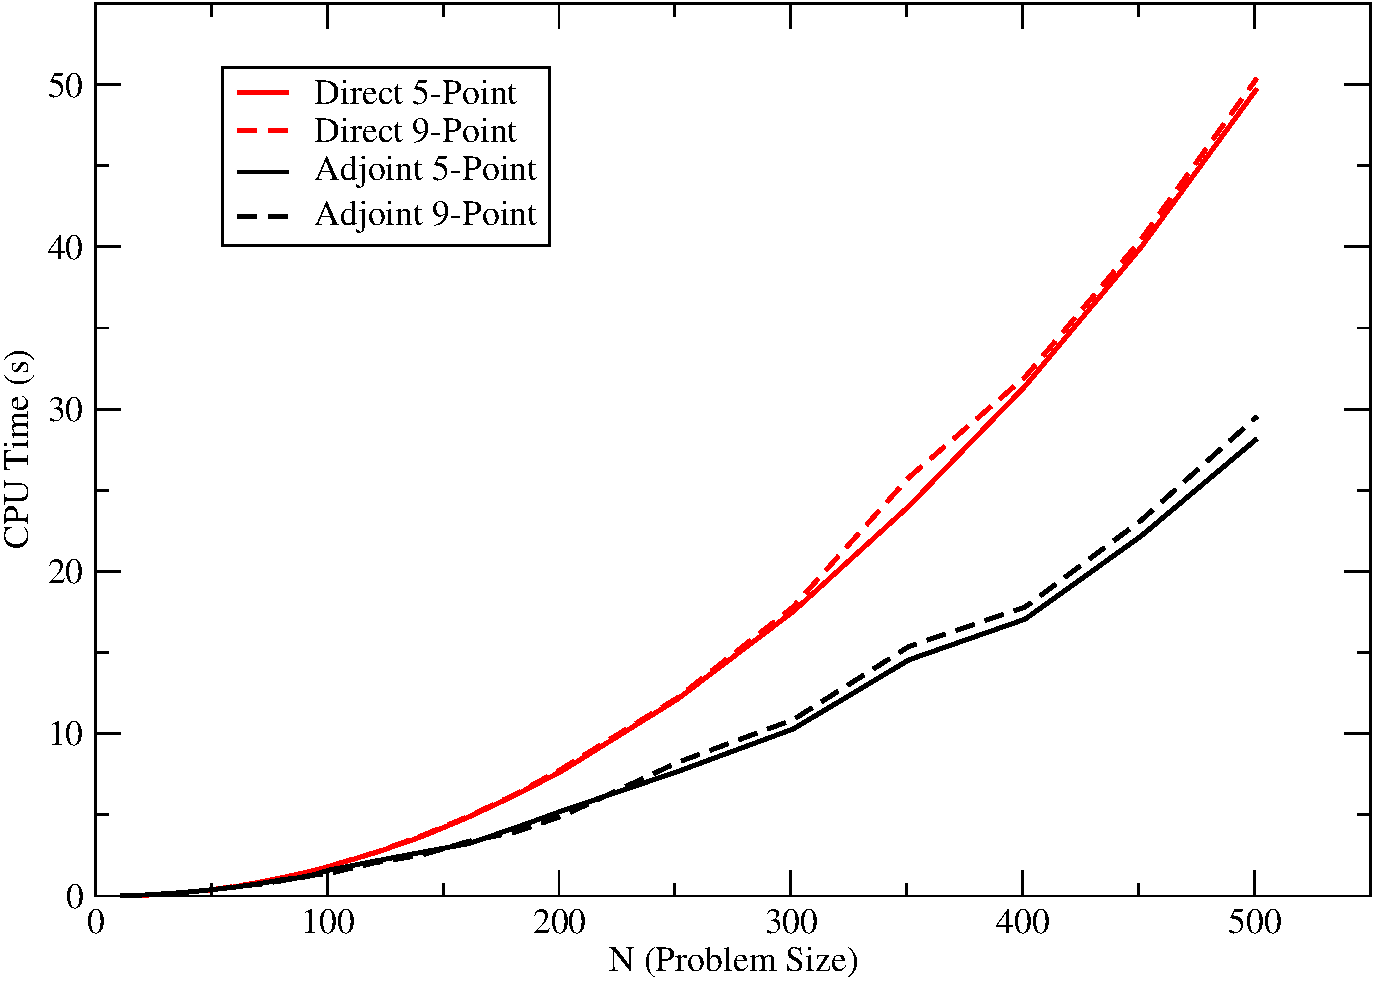
\includegraphics[width=5in,clip]{dir_adj_cpu.pdf}
  \caption{\sl CPU Time (s) to converge vs. Problem Size ($N$ for an
    $N \times N$ square mesh). Both the adjoint and direct solvers are
    used with the five point and nine point stencils. A CPU time
    speedup is noted with the adjoint method due to the higher density
    of random walk events in regions with a large residual.}
  \label{fig:poisson_cpu_time}
\end{figure}

\begin{figure}[ht!]
  \centering
  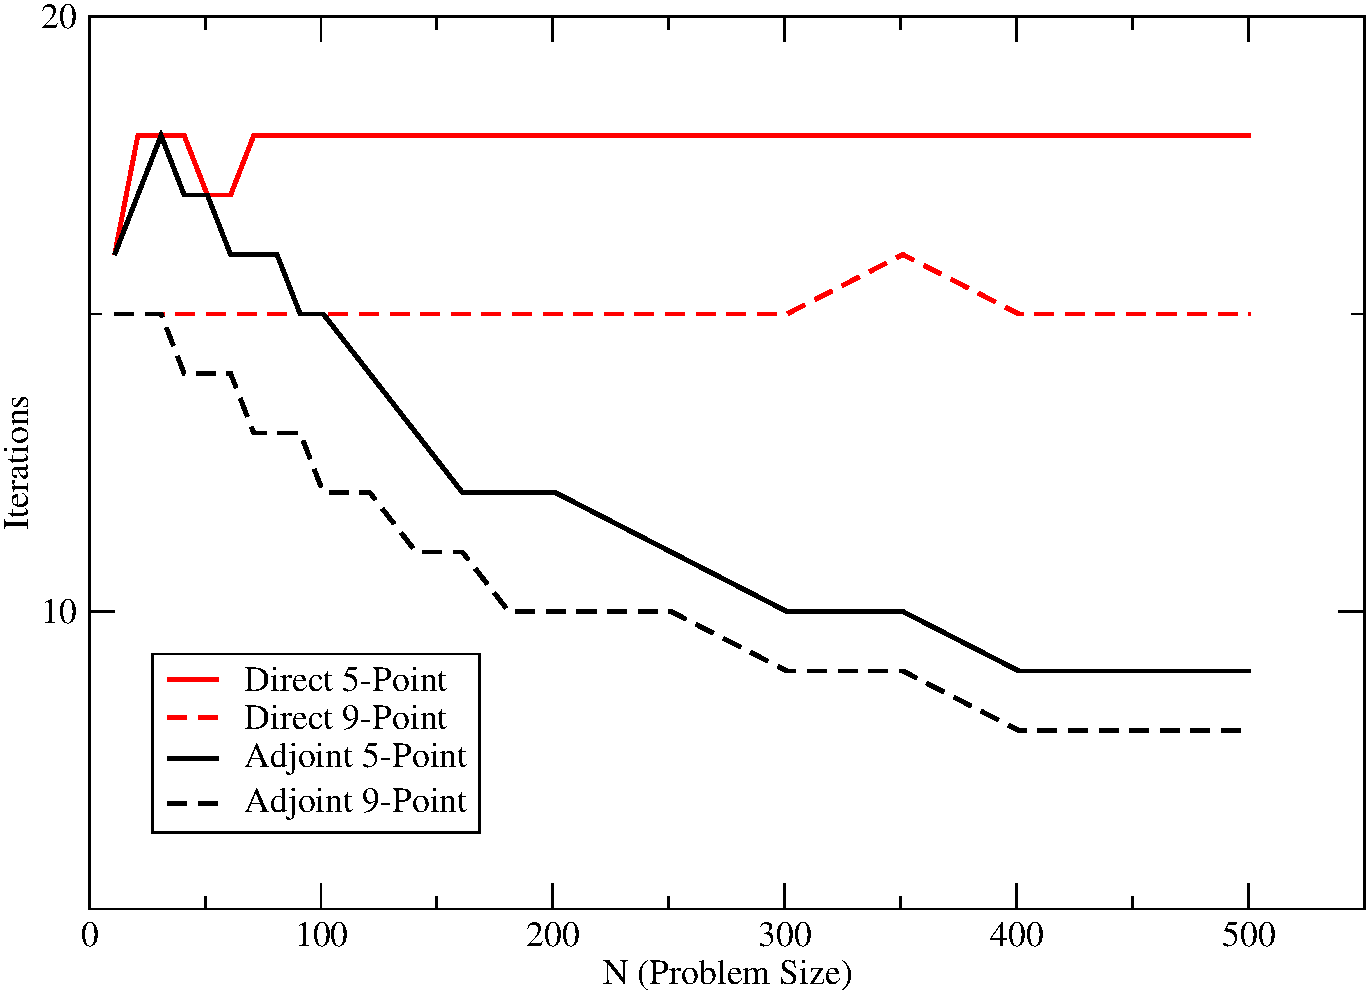
\includegraphics[width=5in,clip]{dir_adj_iterations.pdf}
  \caption{\sl Iterations to converge vs. Problem Size ($N$ for an $N
    \times N$ square mesh). Both the adjoint and direct solvers are
    used with the five-point and nine-point stencils. }
  \label{fig:poisson_iterations}
\end{figure}

We see clearly in Figure~\ref{fig:poisson_cpu_time} that the using the
adjoint solver with MCSA results in a speedup over the direct solver
while the number of iterations required to converge is also reduced as
shown in Figure~\ref{fig:poisson_iterations}. We expect this for several
reasons. First, with an equivalent number of histories specified for
both solvers per MCSA iteration and a system of size $N \times N$, the
direct solver will compute a single random walk for each state in the
system per iteration to acquire a solution in that state, regardless
of the size of the residual in that state. This is necessary in the
direct method to ensure a contribution from each state as the random
walk sequence will only contribute to the starting state. For the
adjoint method, a total of $N \times N$ random walk events will have
their starting state determined by sampling the residual
vector. Because the random walk sequence contributes to the state in
which it currently resides, sampling the residual vector as the Monte
Carlo source gives a higher density of random walk events in regions
with a high residual, thus giving a more accurate correction in that
region due to reduced statistical error. From an iteration
perspective, Figure~\ref{fig:poisson_iterations} shows that using the
direct method yields a roughly unchanging number of iterations
required to converge as the problem size increases. Again, if we
desire a correction value for all states in the problem, then we must
start a random walk in each state in the system which does not reduce
the number of iterations need as the problem size grows. Conversely,
as the problem size grows in the adjoint method, the additional
stochastic histories that will be computed are concentrated in regions
with a large residual, further reducing the stochastic error in the
correction in those regions and subsequently reducing the required
number of iterations to converge.

As an additional comparison, the convergence behavior of MCSA can be
analyzed using both the adjoint and direct solvers to detect any
performance benefits. To assess the convergence properties of MCSA
using each solver and stencil, the infinity norm of the residual
computed in Eq.~(\ref{eq:MCSA-residual}) was collected at each
iteration for a fixed problem size of
$N=500$. Figure~\ref{fig:poisson_convergence} gives the results of
these computations. First, it is worthy to note on the semilog plot
that we are indeed achieving the expected exponential convergence from
MCSA with both Monte Carlo solvers. Second, we note that using the
adjoint method with the same number of stochastic histores per MCSA
iteration gives a faster rate of converge for the same reasons as
above. We also note here that fewer iterations are required for
convergence when the 9-point stencil is used to discretize the
Laplacian operator (although at no gain in speed as given by the
results in Figure~\ref{fig:poisson_cpu_time}). This is due to the fact
that the smaller discretization error directly corresponds to a more
well defined residual source generated by the Richardson extrapolation
for the Monte Carlo calculation. In addition, the better defined
source is transported through a domain described more accurately by
the 9-point stencil, thus yielding a more accuracte correction vector
from the Monte Carlo calculation.
\begin{figure}[ht!]
  \centering
  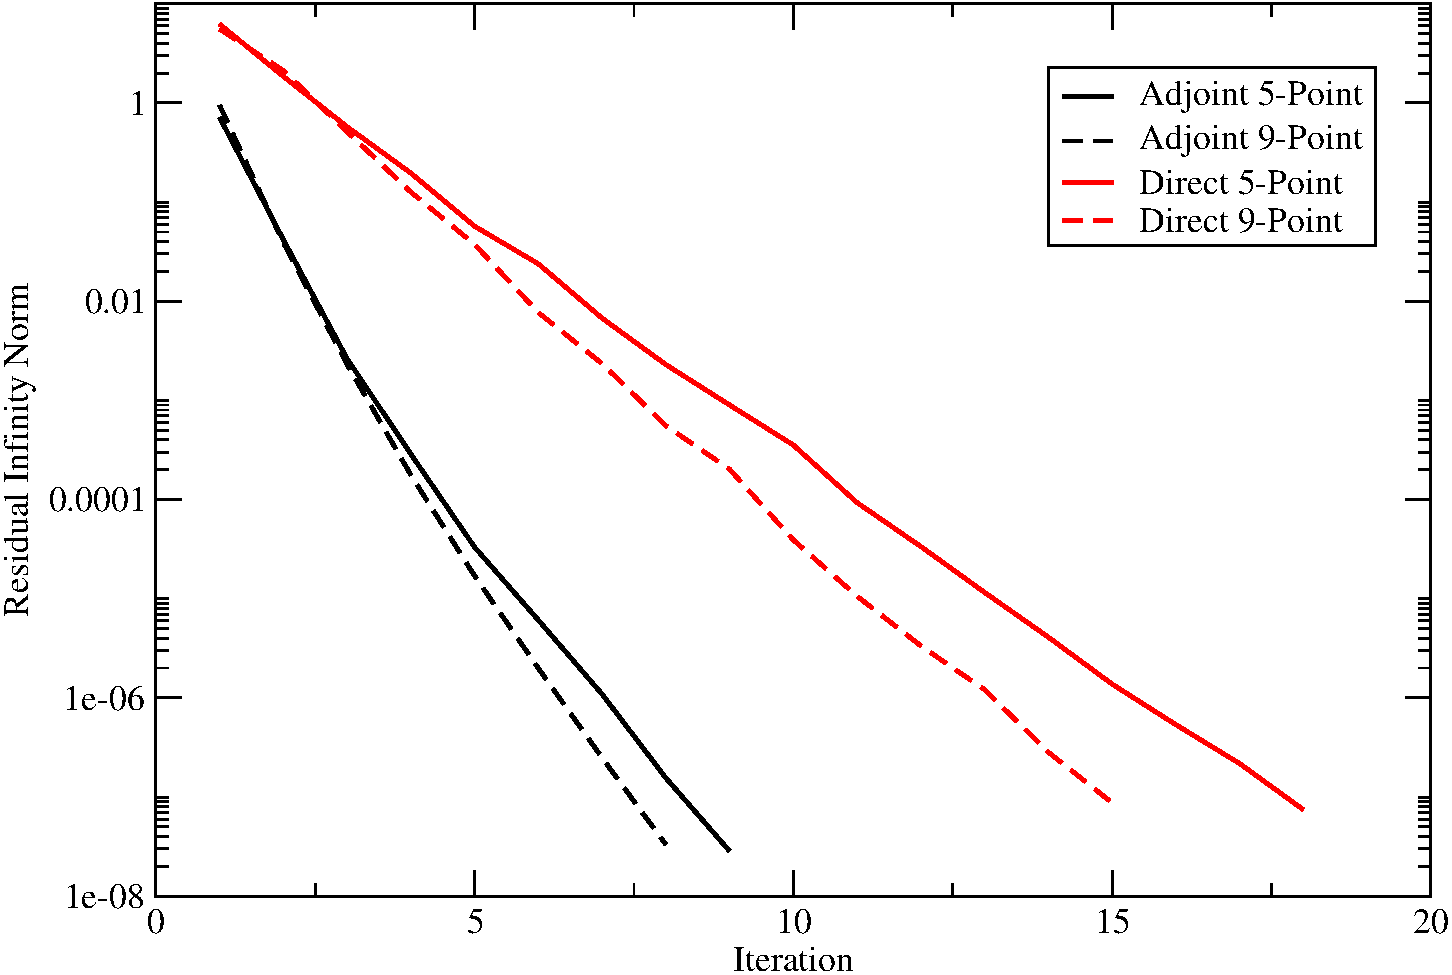
\includegraphics[width=5in,clip]{dir_adj_conv.pdf}
  \caption{\sl Infinity norm of the solution residual vs. iteration
    number for a problem of size $N=500$. Both the adjoint and direct
    solvers are used with the five point and nine point stencils. A
    higher rate of convergence is observed for MCSA using the adjoint
    Monte Carlo solver as compared to the direct method when both
    solvers compute the same number of random walks per iteration.}
  \label{fig:poisson_convergence}
\end{figure}

\subsection{Comparison to Sequential Monte Carlo}
\label{subsec:sequential_comparison}
To further motivate using Monte Carlo Synthetic Acceleration, we
compare its performance to Halton's Sequential Monte Carlo method on
which our previous work in this area was based. For this comparison,
we use the same transient Poisson problem as described in the previous
section and choose only the 5-point stencil to discretize the
Laplacian operator as the previous results yielded little qualitative
difference between the discretizations. Both MCSA and Halton's method
are used with the adjoint Monte Carlo solver. In order to complete the
same study as in the previous section, the number of histories
computed by the Monte Carlo solver at each iteration had to be doubled
to $2 \times N \times N$ in order to ensure convergence in Sequential
Monte Carlo Method. Figure~\ref{fig:seq_cpu_time} gives the CPU time
results for this comparison as a function of problem size while
Figure~\ref{fig:seq_iterations} gives the number of iterations to
converge as a function of problem size. In both cases, using the Monte
Carlo solver as a synthetic acceleration rather than in a pure
residual Monte Carlo scheme resulted in a reduction in both CPU time
and iterations required to converge. The additional Richardson
extrapolation between each Monte Carlo solve in the MCSA method gives
a better converged residual source to use with the Monte Carlo
calculation while the Sequential method requires more iterations to
achieve the same level of convergence in the residual.

\begin{figure}[ht!]
  \centering
  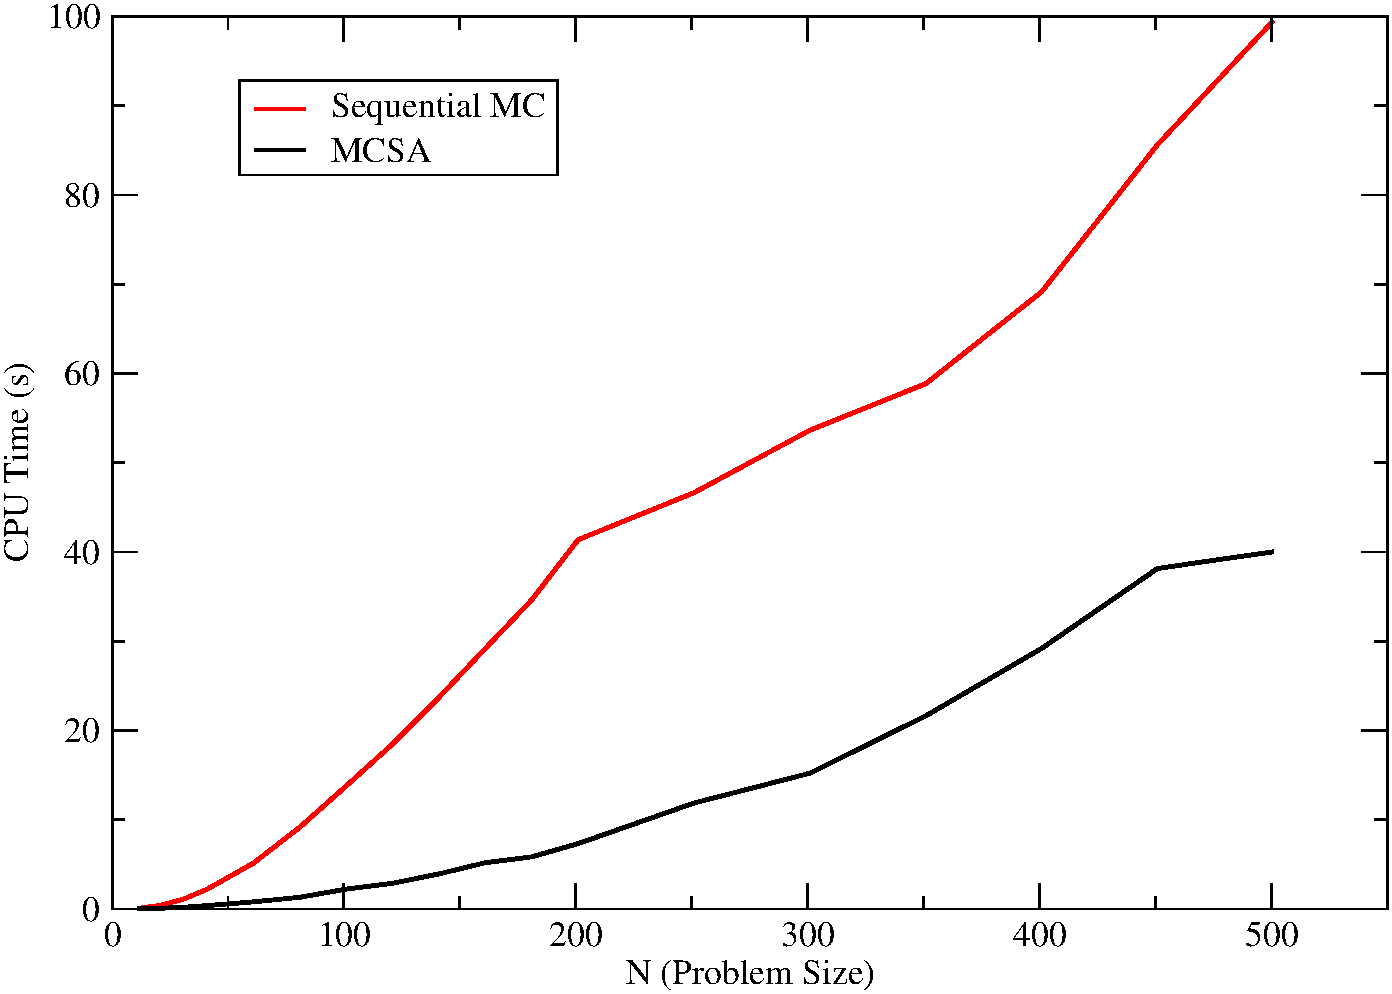
\includegraphics[width=5in,clip]{seq_cpu.pdf}
  \caption{\sl CPU Time (s) to converge vs. Problem Size ($N$ for an
    $N \times N$ square mesh). Both the Sequential Monte Carlo and
    MCSA solvers are used with the five point stencils and the adjoint
    Monte Carlo solver. The number of random walks was twice the
    number of discrete states in the system in order to ensure
    convergence in the Sequential Monte Carlo method.}
  \label{fig:seq_cpu_time}
\end{figure}

\begin{figure}[ht!]
  \centering
  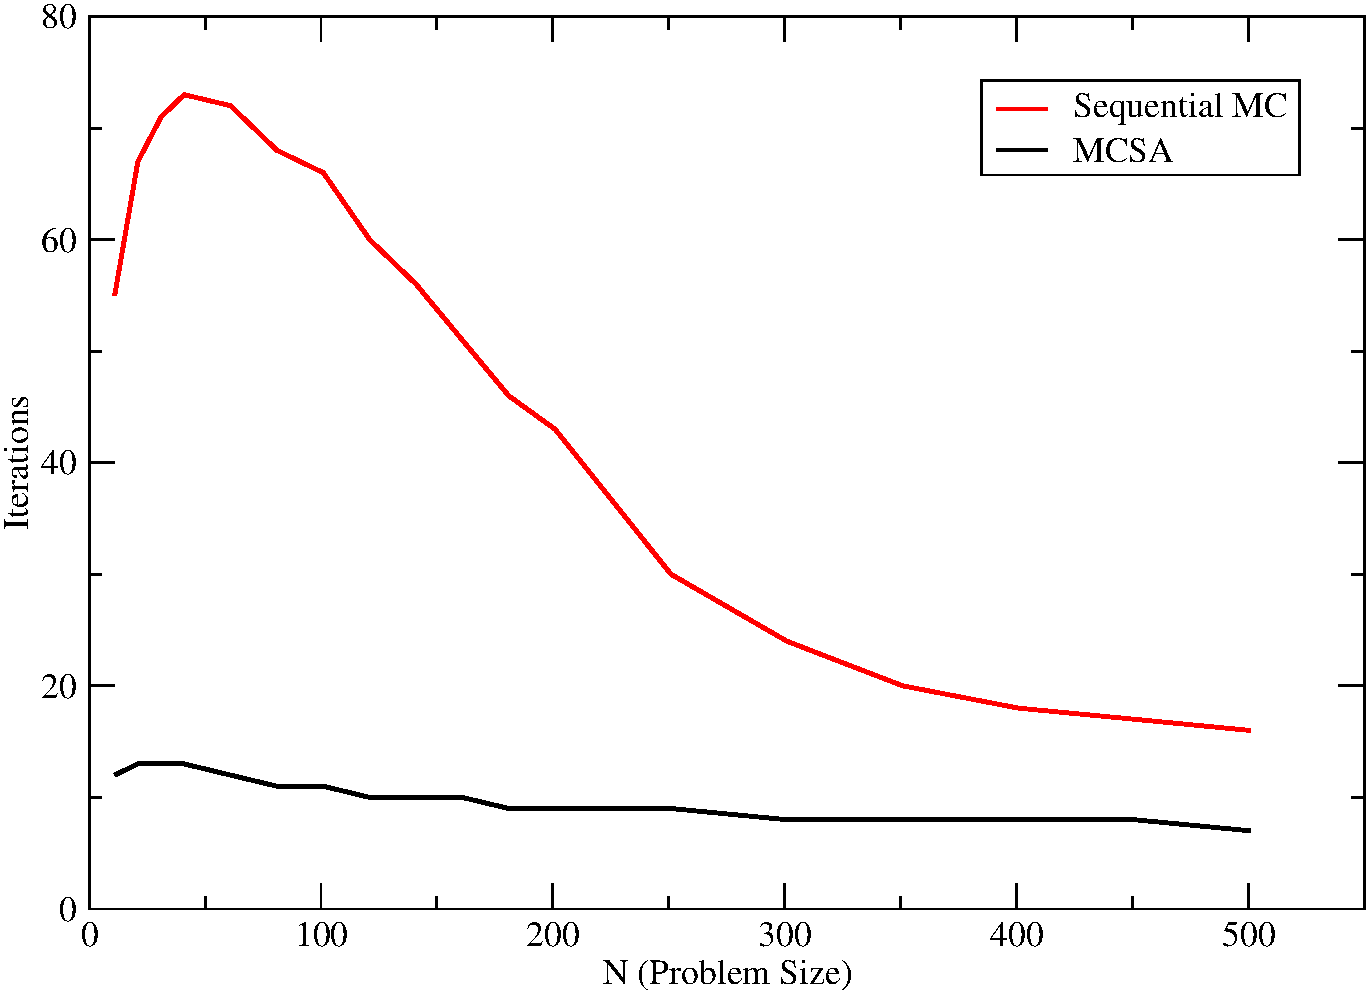
\includegraphics[width=5in,clip]{seq_iterations.pdf}
  \caption{\sl Iterations to converge vs. Problem Size ($N$ for an $N
    \times N$ square mesh). Both the Sequential Monte Carlo and MCSA
    solvers are used with the five point stencils and the adjoint
    Monte Carlo solver.}
  \label{fig:seq_iterations}
\end{figure}

The benefits of using a synthetic acceleration scheme are also noted
when the infinity norm of the residual computed at each iteration for
both methods was collected at each iteration for a fixed problem sizes
of $N=100$ and $N=500$ as shown in figures Figure~\ref{fig:seq_100}
and \ref{fig:seq_500} respectively. In both cases, the Sequential
method is subject to two regimes of exponential convergence with the
later regime converging the slowest while the MCSA method exhibits a
single rate of exponential convergence observed to be much higher than
that computed by Halton's method. Even with the doubling of the number
of stochastic histories computed per time step in order to ensure
convergence for the Sequential method, we still see robustness issues
with a non-monotonically decreasing residual observed for the $N=100$
case. In both cases the MCSA solver is observed to be robust with a
monotonically decreasing residual.

\begin{figure}[ht!]
  \centering
  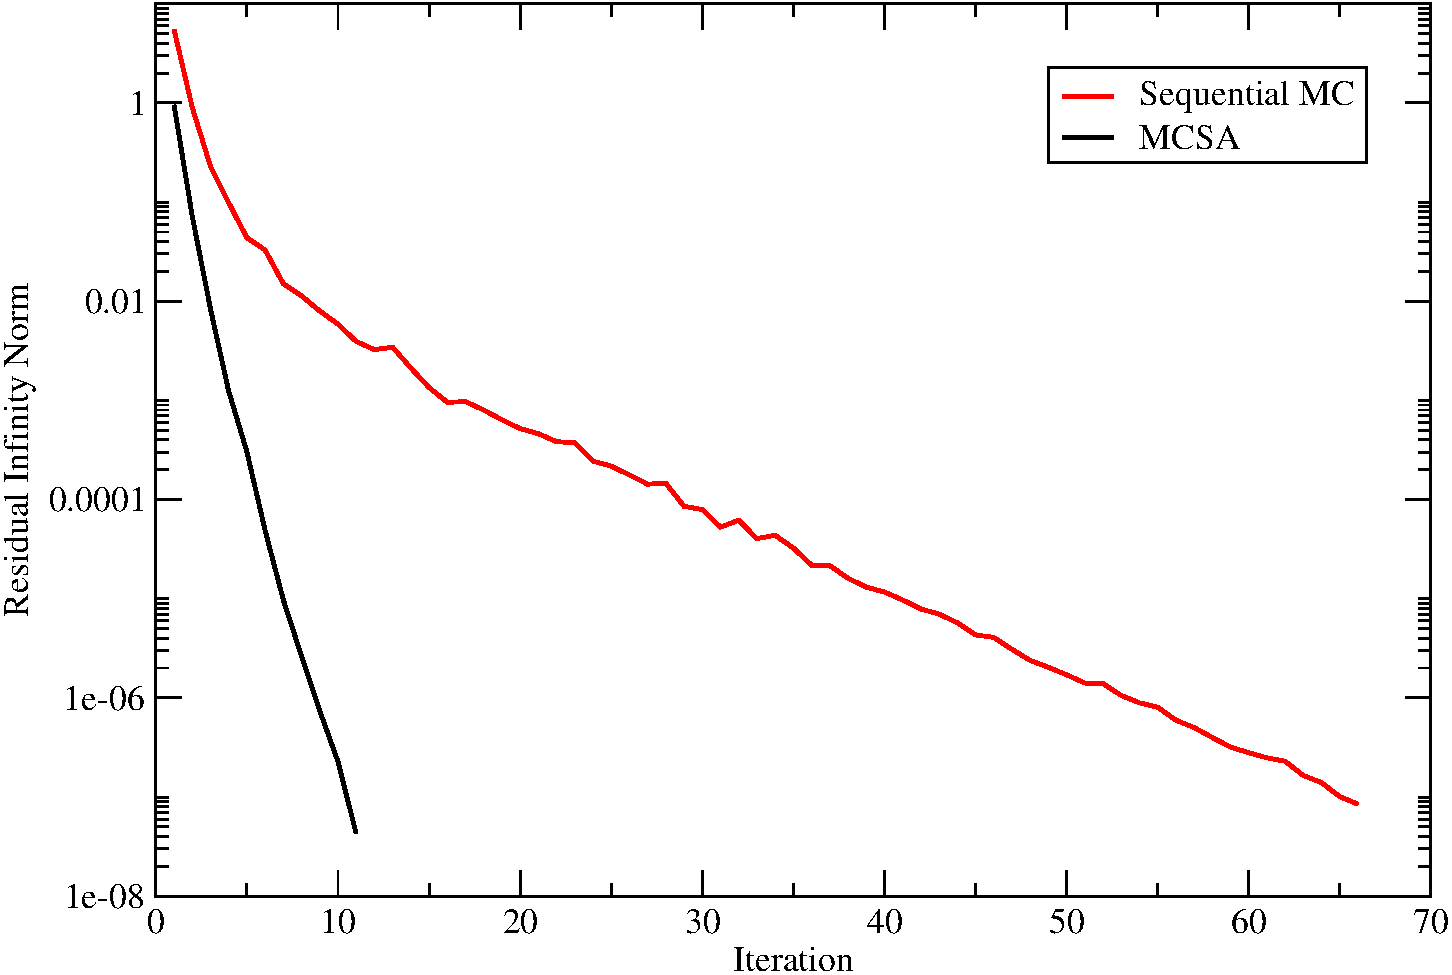
\includegraphics[width=5in,clip]{seq_conv_100.pdf}
  \caption{\sl Infinity norm of the solution residual vs. iteration
    number for a problem of size $N=100$. Both the Sequential Monte
    Carlo and MCSA solvers are used with the five point stencils and
    the adjoint Monte Carlo solver.}
  \label{fig:seq_100}
\end{figure}

\begin{figure}[ht!]
  \centering
  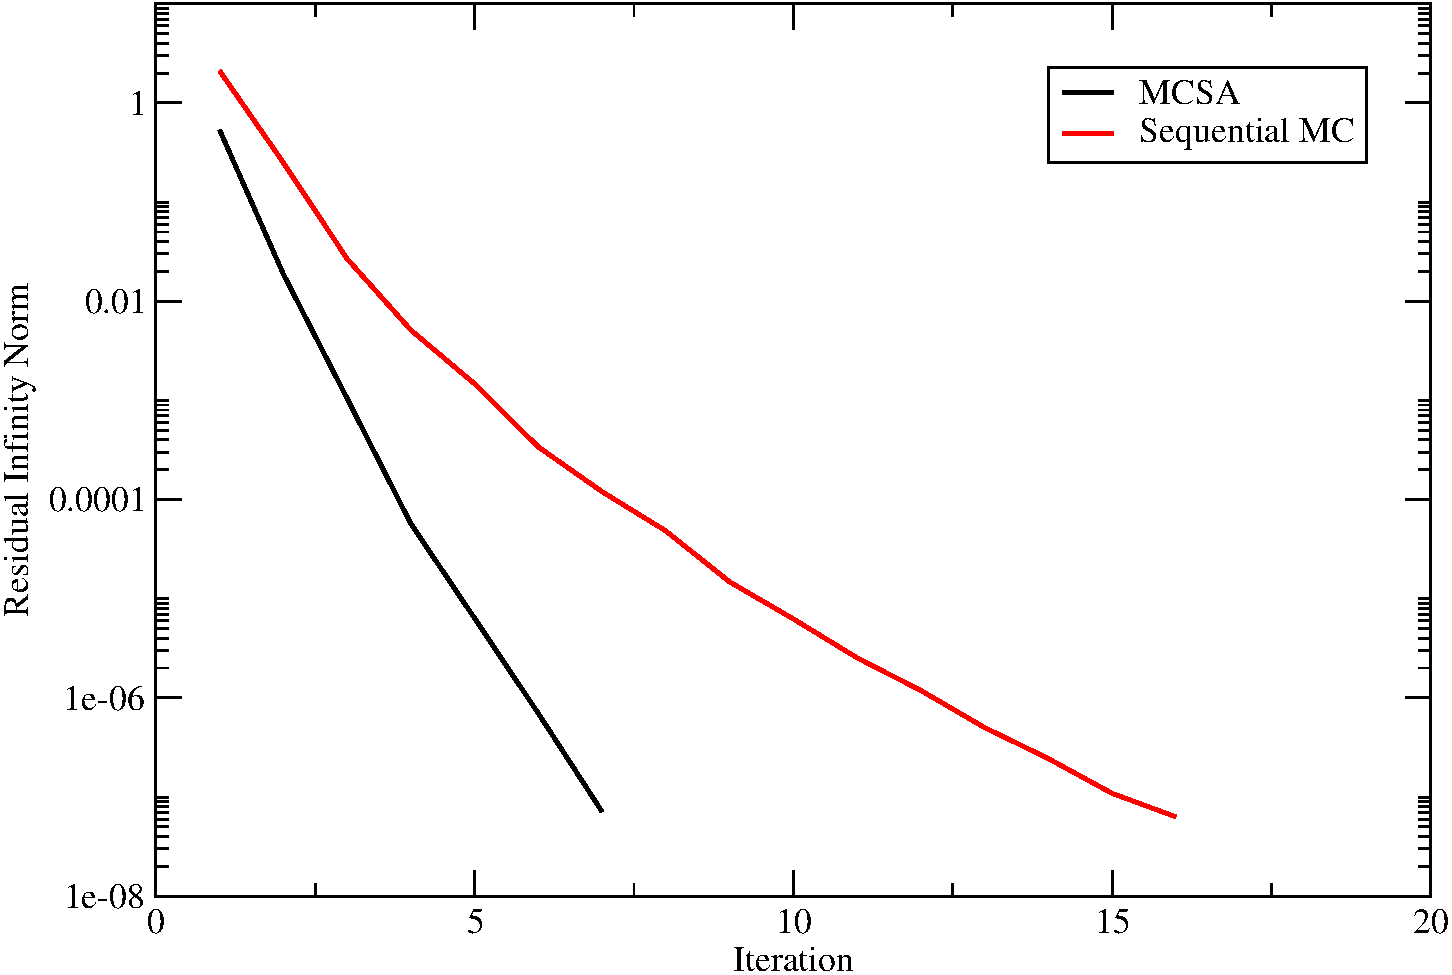
\includegraphics[width=5in,clip]{seq_conv_500.pdf}
  \caption{\sl Infinity norm of the solution residual vs. iteration
    number for a problem of size $N=500$. Both the Sequential Monte
    Carlo and MCSA solvers are used with the five point stencils and
    the adjoint Monte Carlo solver.}
  \label{fig:seq_500}
\end{figure}

%%---------------------------------------------------------------------------%%
\section{Discrete Form of the Radiation Diffusion Equation}
\label{sec:discr-form-radi}

Using the mathematical preliminaries developed in the previous section, we can
now generate a discrete form of the radiation diffusion equation. We will show
that this discrete form is amenable to interpretation using Monte Carlo
concepts and can be written in a way that a random walk sequence can be
generated.

\subsection{Equilibrium Diffusion Model}

The general form of the equilibrium diffusion equation is \cite{morel_1996}
\begin{equation} 
  (\rho\Cv + 4aT^{3})\pder{T}{t} -
  \nabla\cdot{\Bigl(\frac{4acT^{3}}{3\ros}\Bigr)\grad{T}} = Q\:,
  \label{eq:eq-diff-T}
\end{equation}
where $\Cv\equiv\Cv(\ve{r},T(\ve{r},t))$
$[\text{GJ}\cdot\text{g}^{-1}\cdot\text{keV}^{-1}]$ is the specific heat
capacity of the material, $\rho\equiv\rho(\ve{r})$
$[\text{g}\cdot\text{cm}^{-3}]$ is the density of the material, $a=0.01372$
$[\text{GJ}\cdot\text{cm}^{-3}\cdot\text{keV}^{-4}]$ is the radiation
constant, $c=29.979$ $[\text{cm}\cdot\text{ns}^{-1}]$ is the vacuum light
speed, and $T\equiv T(\ve{r},t)$ $[\text{keV}]$ is the temperature that
characterizes both the radiation and the material.  The opacity,
$\ros\equiv\ros$(\ve{r},T(\ve{r},t)) $[\text{cm}^{-1}]$, is the Rosseland Mean
opacity.  The source, $Q\equiv Q(\ve{r},t)$
$[\text{GJ}\cdot\text{cm}^{-3}\cdot\text{ns}^{-1}]$, is assumed to be
independent of $T$.

We choose to use the angle-energy integrated radiation intensity,
$\phi\equiv\phi(\ve{r},t)$
$[\text{GJ}\cdot\text{cm}^{-2}\cdot\text{ns}^{-1}]$, as the primary state
variable.  The intensity is defined as
\begin{equation}
  \label{eq:lte-phi}
  \begin{split}
    \phi(\ve{r},t) &=
    \int_{4\pi}d\bOmega\int_{\nu}d\nu\:\psi(\ve{r},\nu,\hat{\bOmega},t)
    \\ &= \int_{\nu}d\nu\: 4\pi B(\nu,T) \\ &= acT^{4}\:,
  \end{split}
\end{equation}
where $\psi$ is the angular radiation intensity and $\nu$ is the radiation
frequency.  The Planck function (or Planckian) is defined as
\begin{equation}
  B(\nu,T)=\frac{2h\nu^{3}}{c^{2}}\bigl(e^{\frac{h\nu}{kT}} -
  1\bigr)^{-1}\:,
\end{equation}
where $h$ is Planck's constant and $k$ is the Boltzmann constant.  Utilizing
this definition of $\phi$ we can write
\begin{equation}
  \label{eq:partial-T}
  \pder{T}{t} = \frac{1}{4acT^{3}}\pder{\phi}{t}\:.
\end{equation}
Inserting \eqref{eq:partial-T} into \eqref{eq:eq-diff-T} yields
\begin{equation}
  \label{eq:eq-diff}
  \Bigl(\frac{\rho\Cv}{4acT^{3}} + \frac{1}{c}\Bigr)\pder{\phi}{t} -
  \nabla\cdot D\grad{\phi} = Q\:,
\end{equation}
where $D$ is the diffusion coefficient, $D\equiv
D(\ve{r},T(\ve{r},t))\ [\text{cm}]$, and is defined as
\begin{equation}
  D = \frac{1}{3\ros}\:.
\end{equation}
Equation~\eqref{eq:eq-diff} is the model equation we will solve using the
Monte Carlo techniques presented in \S~\ref{sec:monte-carlo-matrix} and
\ref{sec:iter-refin-monte}.

\subsection{Discrete Diffusion Equation}

Applying backward-Euler time differencing to Eq.~(\ref{eq:eq-diff}) and
lagging the temperature-dependent coefficients at $t^n$ gives
\begin{equation}
  -\nabla\cdot \Dn\grad{\phi} + \sign\phi = \qn\:,
\end{equation}
where we have suppressed the $n+1$ indices on $\phi$ and
\begin{align}
  \sign &= \frac{\rho \Cv^n}{4ac(\Tn)^3\dt} + \frac{1}{c\dt}\:,\\ \qn
  &= \sign\phin + Q^n\:,\\ \phin &= ac(\Tn)^4\:.
\end{align}
Applying Fick's Law,
\begin{equation}
  \ve{F} = -D\grad{\phi}\:,
  \label{eq:fick}
\end{equation}
where $\ve{F}$ is the radiation flux, we define a flux-balance equation,
\begin{equation}
  \dive{F} + \sign\phi = \qn\:.
  \label{eq:flux-balance}
\end{equation}
Integrating Eq.~(\ref{eq:flux-balance}) over the cell illustrated in
Figure~\ref{fig:cell} gives
\begin{equation}
  \iiint\dive{F}\,d\ve{r} +
  \sign_{ijk}\phi_{ijk}V_{ijk}=\qn_{ijk}V_{ijk}\:,
  \label{eq:flux-balance-vol-integral}
\end{equation}
and $V_{ijk} = \Delta_i\Delta_j\Delta_k$.
\begin{figure}[ht!]
  \centerline{ 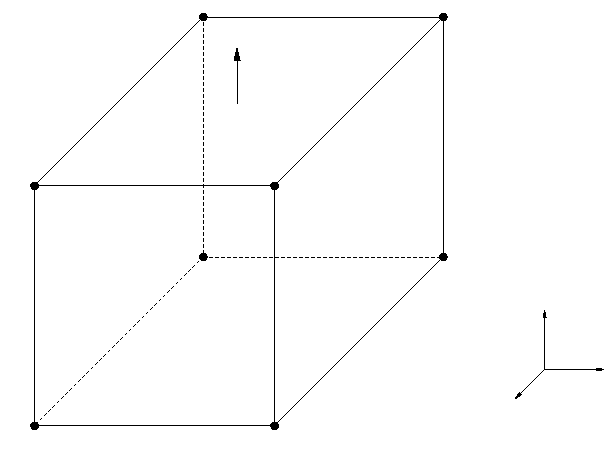
\includegraphics[clip]{mesh_cell.pdf} }
  \caption{Orthogonal 3D mesh cell.}
  \label{fig:cell}
\end{figure}
We now apply the divergence theorem,
\begin{equation}
  \begin{split}
    \iiint\dive{F}\,d\ve{r} &= \oint\hat{\ve{n}}\cdot\ve{F}\,dA\\ &=
    \sum_{f=1}^{6}\hat{\ve{n}}_f\cdot\ve{F}_f A_f\:,
  \end{split}
\end{equation}
to Eq.(\ref{eq:flux-balance-vol-integral}) yielding
\begin{equation}
  \begin{split}
    (F_{i+1/2} - F_{i-1/2})\Dj\Dk &+ (F_{j+1/2} - F_{j-1/2})\Di\Dk +
    (F_{k+1/2}\\ &- F_{k-1/2})\Di\Dj + \sign_{ijk}\phi_{ijk}V_{ijk} =
    \qn_{ijk}V_{ijk}\:.
  \end{split}
  \label{eq:flux-balance-difference}
\end{equation}

Using Fick's Law, Eq.~(\ref{eq:fick}), we can write $O(\Delta^2)$ expressions
for the face-centered fluxes.  Defining $l\in\{i,j,k\}$, the face-centered
fluxes are
\begin{align}
  F_{l+1/2} &= -D_{l+1/2}\frac{\phi_{l+1} -
    \phi_{l}}{\Delta_{l+1/2}}\:, \label{eq:F_l+1/2}\\ F_{l-1/2} &=
  -D_{l-1/2}\frac{\phi_{l} -
    \phi_{l-1}}{\Delta_{l-1/2}}\:, \label{eq:F_l-1/2}
\end{align}
where
\begin{align}
  \Delta_{l+1/2} &= \frac{\Delta_{l+1} +
    \Delta_{l}}{2}\:,\\ \Delta_{l-1/2} &= \frac{\Delta_{l} +
    \Delta_{l-1}}{2}\:.
\end{align}
In order to be conservative, the flux must be continuous across a face.  Thus,
the face-centered flux evaluated from either side of the face must be
equivalent:
\begin{equation}
  \begin{aligned}
    F_{l+1/2}^{+} &= F_{l+1/2}^{-}\:,\\ 2D_{l+1}\frac{\phi_{l+1} -
      \phi_{l+1/2}}{\Delta_{l+1}} &= 2D_{l}\frac{\phi_{l+1/2} -
      \phi_{l}}{\Delta_l}\:,\\ \frac{1}{3\sigma_{l+1}}\frac{\phi_{l+1}
      - \phi_{l+1/2}}{\Delta_{l+1}} &=
    \frac{1}{3\sigma_{l}}\frac{\phi_{l+1/2} - \phi_{l}}{\Delta_l}\:,
  \end{aligned}
\end{equation}
where we have dropped the subscript $\mathrm{R}$ from $\sigma$ for clarity.
Solving this system for $\phi_{l+1/2}$ and applying to either $F_{l+1/2}^{+}$
or $F_{l+1/2}^{-}$ and setting the resulting expression equal to
Eq.~(\ref{eq:F_l+1/2}), one finds the face-centered diffusion coefficient,
\begin{equation}
  D_{l+1/2} = \frac{2\Delta_{l+1/2}}{3\sigma_l\Delta_l +
    3\sigma_{l+1}\Delta_{l+1}}\:.
  \label{eq:D_l+1/2}
\end{equation}
Following the same procedure at the $l-1/2$ face gives the diffusion
coefficient on the low-side face:
\begin{equation}
  D_{l-1/2} = \frac{2\Delta_{l-1/2}}{3\sigma_l\Delta_l +
    3\sigma_{l-1}\Delta_{l-1}}\:.
  \label{eq:D_l-1/2} 
\end{equation}

Using Eqs.~(\ref{eq:F_l+1/2}), (\ref{eq:F_l-1/2}), (\ref{eq:D_l+1/2}),
and (\ref{eq:D_l-1/2}) in the discrete flux-balance equation,
(\ref{eq:flux-balance-difference}), we obtain
\begin{equation}
  \begin{aligned}
    \sigT\phi_{ijk} -
    \sigm_{i+1}\frac{\Delta_{i+1}}{\Di}\phi_{i+1\,jk} & -
    \sigp_{i-1}\frac{\Delta_{i-1}}{\Di}\phi_{i-1\,jk}\\ &-
    \sigm_{j+1}\frac{\Delta_{j+1}}{\Dj}\phi_{i\,j+1\,k} -
    \sigp_{j-1}\frac{\Delta_{j-1}}{\Dj}\phi_{i\,j-1\,k}\\ &-
    \sigm_{k+1}\frac{\Delta_{k+1}}{\Dk}\phi_{ij\,k+1} -
    \sigp_{k-1}\frac{\Delta_{k-1}}{\Dk}\phi_{ij\,k-1} = \qn_{ijk}\:.
  \end{aligned}
  \label{eq:discrete-diffusion}
\end{equation}
Here,
\begin{equation}
  \sigT = \sigp_i + \sigm_i + \sigp_j + \sigm_j + \sigp_k + \sigm_k +
  \sign_{ijk}\:,
\end{equation}
and
\begin{subequations}
  \begin{align}
    \sigp_{i} &= \frac{1}{\Di}\frac{2}{3\sigma_{ijk}\Di +
      3\sigma_{i+1\,jk}\Delta_{i+1}}\:,\\ \sigm_{i} &=
    \frac{1}{\Di}\frac{2}{3\sigma_{ijk}\Di +
      3\sigma_{i-1\,jk}\Delta_{i-1}}\:,\\ \sigp_{j} &=
    \frac{1}{\Dj}\frac{2}{3\sigma_{ijk}\Dj +
      3\sigma_{i\,j+1\,k}\Delta_{j+1}}\:,\\ \sigm_{j} &=
    \frac{1}{\Dj}\frac{2}{3\sigma_{ijk}\Dj +
      3\sigma_{i\,j-1\,k}\Delta_{j-1}}\:,\\ \sigp_{k} &=
    \frac{1}{\Dk}\frac{2}{3\sigma_{ijk}\Dk +
      3\sigma_{ij\,k+1}\Delta_{k+1}}\:,\\ \sigm_{k} &=
    \frac{1}{\Dk}\frac{2}{3\sigma_{ijk}\Dk +
      3\sigma_{ij\,k-1}\Delta_{k-1}}\:.
  \end{align}
  \label{eq:sigmas}
\end{subequations}
Also, note that
\begin{align*}
  \sigp_{i-1} &= \frac{1}{\Delta_{i-1}}\frac{2}{3\sigma_{ijk}\Di +
    3\sigma_{i-1\,jk}\Delta_{i-1}}\:,\\ \sigm_{i+1} &=
  \frac{1}{\Delta_{i+1}}\frac{2}{3\sigma_{ijk}\Di +
    3\sigma_{i+1\,jk}\Delta_{i+1}}\:,\\ \ldots\:.
\end{align*}
Equations~(\ref{eq:discrete-diffusion}) through (\ref{eq:sigmas}) represent
the discretized, 1T diffusion equation on an orthogonal 3D grid.

Equations~(\ref{eq:discrete-diffusion}) through (\ref{eq:sigmas}) have been
written in a manner that is amenable to Monte Carlo interpretation.  One can
envision the terms in Eq.~(\ref{eq:sigmas}) representing leakage out of each
face of a cell.  The off-diagonal terms then represent sources into the cell,
or, equivalently, these terms are leakage out of the neighboring cells.  A
limitation of this interpretation is that it requires a symmetric system to
implement the Monte Carlo scheme.  More specifically, the operator $\ve{D}$
must be an H-matrix \cite{kelley_1995} such that the off-diagonal elements are
negative and symmetric.  In other words, the leakage out of a cell must be
equivalent to the source into the adjacent cell.

The methods described in \S\S~\ref{sec:monte-carlo-matrix} and
\ref{sec:iter-refin-monte} do not suffer this limitation.  Thus, we will
interpret the solution via MCSA as a transport-like process, but we do not
require any constraints on the system other than the spectral radius must be
less than 1.

Before completing the derivation of discrete equations required to solve
Eq.~(\ref{eq:discrete-diffusion}), we must specify boundary conditions.  For
this work, the Marshak Boundary condition suffices:
\begin{equation}
  f_b^\pm = \frac{1}{4}\phi -
  \frac{1}{2}\ve{F}\cdot\hat{\ve{n}}\:,\quad \vr\in \partial\Gamma\:,
\end{equation}
where $f_b$ is the incoming partial current on the problem boundary,
$\partial\Gamma$.  On any low boundary we can write the flux using a
first-order discrete form of Fick's Law:
\begin{equation}
  F_{1/2} = -\frac{2}{3\sigma_1}\frac{\phi_1 -
    \phi_{1/2}}{\Delta_1}\:.
  \label{eq:low-boundary-flux}
\end{equation}
As before, we enforce continuity of flux on the boundary using the
Marshak Boundary condition:
\begin{equation}
  -\frac{2}{3\sigma_1}\frac{\phi_1 - \phi_{1/2}}{\Delta_1} = 2f_b^{+}
  -\frac{1}{2}\phi_{1/2}\:.
\end{equation}
Solving for $\phi_{1/2}$ and applying to Eq.~(\ref{eq:low-boundary-flux})
yields an expression for the low-side boundary flux:
\begin{equation}
  F_{1/2} = \frac{2}{3\sigma_1\Delta_1 + 4}(4f_b^{+}-\phi_1)\:.
\end{equation}
Following an identical procedure on high-side problem boundaries gives
\begin{equation}
  F_{N_l+1/2} = \frac{2}{3\sigma_{N_l}\Delta_{N_l} +
    4}(\phi_{N_l}-4f_b^{-})\:,
\end{equation}
where $l\in\{i,j,k\}$ is defined over the range $[1,N_l]$.

These boundary fluxes take the place of the interior face-centered fluxes
(defined in Eqs.~(\ref{eq:F_l+1/2}) and (\ref{eq:F_l-1/2})) in
Eq.~(\ref{eq:flux-balance-difference}) yielding the following modifications to
Eqs.~(\ref{eq:sigmas}) on a boundary:
\begin{align}
  \text{low boundary:}\quad & \sigma_1^{-} = \frac{1}{\Delta_1}
  \frac{2}{3\sigma_1\Delta_1 + 4}\:,\\ \text{high boundary:}\quad &
  \sigma_{N_l}^{+} = \frac{1}{\Delta_{N_l}}
  \frac{2}{3\sigma_{N_l}\Delta_{N_l} + 4}\:.
\end{align}
Furthermore, the following contributions are added to the source, $\qn_{ijk}$
on a boundary cell:
\begin{align}
  \text{low boundary:}\quad & \frac{8}{\Delta_1}
  \frac{1}{3\sigma_1\Delta_1 + 4}f_b^{+}\:,\\ \text{high
    boundary:}\quad & \frac{8}{\Delta_{N_l}}
  \frac{1}{3\sigma_{N_l}\Delta_{N_l} + 4}f_b^{-}\:.
\end{align}
Note that for vacuum boundary conditions, $f_b^{\pm} = 0$.

For reflective boundary conditions we have the simple modification that
\begin{align}
  F_{1/2} &= 0\:, \\ F_{N_l+1/2} &= 0\:.
\end{align}
Thus, there are no leakage or adjacent cell source terms resulting from this
boundary face.

\subsection{Preconditioning}
\label{sec:preconditioning}

The discrete diffusion equation in (\ref{eq:discrete-diffusion}) can be
written in matrix-operator form as follows:
\begin{equation}
  \ve{D}\bphi = \ve{q}\:,
  \label{eq:diffusion-matrix}
\end{equation}
where $\ve{D}$ is a symmetric, positive-definite (SPD) operator.
Unfortunately, for many problems $\rho(\ve{D}) > 1$.  Therefore, we must
precondition Eq.~(\ref{eq:diffusion-matrix}) in order to use the MCSA
method. We apply left-preconditioning and write
\begin{equation}
  \ve{M}^{-1}\ve{D}\bphi = \ve{M}^{-1}\ve{q}\:.
  \label{eq:preconditioned-diffusion}
\end{equation}
A good choice for the preconditioner, $\ve{M}$, is to use Jacobi
preconditioning:
\begin{equation}
  \ve{M}=\diag(\ve{D})\:.
  \label{eq:preconditioner}
\end{equation}
Setting $\ve{M}$ equal to the diagonal elements of $\ve{D}$ accomplishes
several objectives:
\begin{itemize}
\item For diagonally dominant systems like Eq.~(\ref{eq:diffusion-matrix}), it
  reduces the spectral radius such that $\rho(\ve{M}^{-1}\ve{D}) <
  \rho(\ve{D})$ and $\rho(\ve{M}^{-1}\ve{D}) < 1$ \cite{golub}.  Thus,
  convergence is guaranteed and fewer iterations are required, resulting in
  accelerated convergence.
\item The diagonal elements of the preconditioned iteration matrix are zero:
  $\diag(\vI - \ve{M}^{-1}\ve{D}) = 0$.  Thus, there will be no computations
  wasted for in-state transitions $i\rightarrow i$ during the random walk
  process.
\end{itemize}
The second item is quite important for Monte Carlo solutions of linear
systems, and this type of scaling should be performed regardless of any
additional preconditioner choices. 

An advantage of MCSA is that the resulting system does not have to be SPD;
thus, any suitable choice of $\ve{M}$ will suffice.  The preconditioned system
we will solve is defined in Eq.~(\ref{eq:preconditioned-diffusion}).  Applying
$\ve{M}^{-1}$ to Eq.~(\ref{eq:discrete-diffusion}) yields
\begin{equation}
  \begin{aligned}
    \phi_{ijk} -
    \frac{\sigm_{i+1}}{\sigT}\frac{\Delta_{i+1}}{\Di}&\phi_{i+1\,jk} -
    \frac{\sigp_{i-1}}{\sigT}\frac{\Delta_{i-1}}{\Di}\phi_{i-1\,jk}\\ &-
    \frac{\sigm_{j+1}}{\sigT}\frac{\Delta_{j+1}}{\Dj}\phi_{i\,j+1\,k}
    -\frac{\sigp_{j-1}}{\sigT}\frac{\Delta_{j-1}}{\Dj}\phi_{i\,j-1\,k}\\ &-
    \frac{\sigm_{k+1}}{\sigT}\frac{\Delta_{k+1}}{\Dk}\phi_{ij\,k+1} -
    \frac{\sigp_{k-1}}{\sigT}\frac{\Delta_{k-1}}{\Dk}\phi_{ij\,k-1} =
    \frac{\qn_{ijk}}{\sigT}\:.
  \end{aligned}
  \label{eq:preconditioned-discrete-diffusion}
\end{equation}

%%---------------------------------------------------------------------------%%
\section{Solution of the Radiation Diffusion Equation}
\label{sec:solut-radi-diff}

Here we derive the equations required to solve
Eq.~(\ref{eq:preconditioned-discrete-diffusion}) using the MCSA method.  As
discussed in \S~\ref{sec:iter-refin-monte}, the MCSA method requires two
solutions:
\begin{enumerate}
\item A fixed-point iteration to estimate $\bphi^{l+1/2}$.  This is a
  matrix-vector multiply operation.
\item An adjoint Monte Carlo solve to estimate $\delta\bphi^{l+1/2}$.
\end{enumerate}
For clarity, we rewrite the iteration scheme in Eq.~(\ref{eq:MCSA-iteration})
using the diffusion operator notation from
Eq.~(\ref{eq:preconditioned-diffusion}):
\begin{align*}
   \bphi^{l+1/2} = (\vI - \ve{M}^{-1}\ve{D})\bphi^{l} +
  \ve{M}^{-1}\ve{q}\:, \quad & (\text{fixed-point iteration})\\
  %%
  \vr^{l+1/2} = \ve{M}^{-1}\ve{q} - \ve{M}^{-1}\ve{D}\bphi^{l+1/2}\:,
  \quad & (\text{compute residual})\\ 
  %%
  \ve{M}^{-1}\hat{\ve{D}}\delta\bphi^{l+1/2} = \vr^{l+1/2}\:, \quad&
  (\text{estimate $\delta\phi$ using adjoint Monte Carlo method})\\
  %%
  \bphi^{l+1} = \bphi^{l+1/2} + \delta\bphi^{l+1/2}\:. \quad&
  (\text{update}\ \bphi)
\end{align*}
As described in \S~\ref{sec:iter-refin-monte}, the adjoint Monte Carlo method
only approximately inverts $\ve{M}^{-1}\hat{\ve{D}}$ as indicated by the
$\hat{\cdot}$ notation.  We now describe each of these in turn.

First, we use Eq.~(\ref{eq:preconditioned-discrete-diffusion}) to evaluate
$\bphi^{l+1/2}$ via a single fixed-point iteration as follows:
\begin{equation}
  \begin{aligned}
    \phi_{ijk}^{l+1/2} =
    \frac{\sigm_{i+1}}{\sigT}\frac{\Delta_{i+1}}{\Di}&\phi_{i+1\,jk}^l
    +
    \frac{\sigp_{i-1}}{\sigT}\frac{\Delta_{i-1}}{\Di}\phi_{i-1\,jk}^l
    \\ &+
    \frac{\sigm_{j+1}}{\sigT}\frac{\Delta_{j+1}}{\Dj}\phi_{i\,j+1\,k}^l
    +
    \frac{\sigp_{j-1}}{\sigT}\frac{\Delta_{j-1}}{\Dj}\phi_{i\,j-1\,k}^l
    \\ &+
    \frac{\sigm_{k+1}}{\sigT}\frac{\Delta_{k+1}}{\Dk}\phi_{ij\,k+1}^l
    +
    \frac{\sigp_{k-1}}{\sigT}\frac{\Delta_{k-1}}{\Dk}\phi_{ij\,k-1}^l
    + \frac{\qn_{ijk}}{\sigT}\:.
  \end{aligned}
\end{equation}
This result is used to compute the residual of the system.  The residual then
becomes the source for the Monte Carlo simulation.

The adjoint Monte Carlo method described in \S~\ref{sec:adjoint-method} is
used to estimate
\begin{equation}
  \ve{M}^{-1}\hat{\ve{D}}\delta\bphi^{l+1/2} = \vr^{l+1/2}\:.
\end{equation}
As noted above, the residual acts as the source for this simulation, and the
operator $\ve{M}^{-1}\hat{\ve{D}}$ is implicitly defined in
Eq.~(\ref{eq:preconditioned-discrete-diffusion}).  There are two Monte Carlo
interpretations that can be applied to this system.  The first follows the
mathematical presentation given in \S~\ref{sec:monte-carlo-matrix}.  Namely,
we form probabilities from the iteration matrix and perform random walks to
generate unbiased estimates of the solution vector, $\delta\bphi^{l+1/2}$,
using the estimator in Eq.~(\ref{eq:adjoint-tally}).

However, a more natural interpretation for Monte Carlo transport practitioners
is to use the machinery described in \S~\ref{sec:monte-carlo-matrix} to define
Probability Distribution Functions (PDF) that describe the transport of
particles between cells.  We then do a Monte Carlo transport calculation using
Eq.~(\ref{eq:adjoint-weight}) to calculate the weight change at each
collision. Equation~(\ref{eq:adjoint-probability}) gives the probability of
scattering to an adjacent cell. We tally the contribution of $\phi$ in each
cell using Eq.~(\ref{eq:adjoint-tally}).  The transport is terminated using a
relative weight cutoff that is defined in Eq.~(\ref{eq:weight_cutoff}).  We
now examine each of these in more detail.

The connectivity of an arbitrary cell is illustrated in the 3D mesh segment in
Figure~\ref{fig:mesh_segment}.  For a particle residing in the blue cell, any
collision results in a scatter to one of the six adjacent cells since
$p_{ii}=0$ in the preconditioned system.  We can easily calculate the
probabilities for each scattering event from
Eq.~(\ref{eq:preconditioned-discrete-diffusion}) without explicitly forming
the iteration matrix.  In this mesh cell, the probabilities for leakage out of
each face are derived from the equations from each adjacent cell.  Using
Eq.~(\ref{eq:preconditioned-discrete-diffusion}) we can explicitly write the
equations from each adjacent cell, here only noting the contribution from cell
7:
\begin{align*}
  \phi_1 &= \frac{\sigm_{7\rightarrow 1}}{\sigma_{T\,1}}
  \frac{\Delta_7}{\Delta_1}\phi_7 + \ldots\:,\\ 
  %%
  \phi_2 &= \frac{\sigp_{7\rightarrow 2}}
  {\sigma_{T\,2}}\frac{\Delta_7}{\Delta_2}\phi_7 + \ldots\:,\\
  %%
  \phi_3 &= \frac{\sigm_{7\rightarrow 3}}{\sigma_{T\,3}}
  \frac{\Delta_7}{\Delta_3}\phi_7 + \ldots\:,\\ 
  %%
  \phi_4 &= \frac{\sigp_{7\rightarrow 4}}{\sigma_{T\,4}}
  \frac{\Delta_7}{\Delta_4}\phi_7 + \ldots\:,\\
  %%
  \phi_5 &= \frac{\sigm_{7\rightarrow 5}}{\sigma_{T\,5}}
  \frac{\Delta_7}{\Delta_5}\phi_7 + \ldots\:,\\
  %%
  \phi_6 &= \frac{\sigp_{7\rightarrow 6}}{\sigma_{T\,6}}
  \frac{\Delta_7}{\Delta_6}\phi_7 + \ldots\:.\\ 
\end{align*} 
A quick view of these equations reveals that the only non-zero entries in
column 7 of the iteration matrix are
\begin{equation*}
  \begin{pmatrix}
    h_{1,7} & h_{2,7} & h_{3,7} & h_{4,7} & h_{5,7} & h_{6,7}
  \end{pmatrix}^{T}
  =
  \begin{pmatrix}
    \frac{\sigm_{7\rightarrow
        1}}{\sigma_{T\,1}}\frac{\Delta_7}{\Delta_1}
    \\ \frac{\sigp_{7\rightarrow
        2}}{\sigma_{T\,2}}\frac{\Delta_7}{\Delta_2}
    \\ \frac{\sigm_{7\rightarrow
        3}}{\sigma_{T\,3}}\frac{\Delta_7}{\Delta_3}
    \\ \frac{\sigp_{7\rightarrow
        4}}{\sigma_{T\,4}}\frac{\Delta_7}{\Delta_4}
    \\ \frac{\sigm_{7\rightarrow
        5}}{\sigma_{T\,5}}\frac{\Delta_7}{\Delta_5}
    \\ \frac{\sigp_{7\rightarrow
        6}}{\sigma_{T\,6}}\frac{\Delta_7}{\Delta_6}
  \end{pmatrix}\:,
\end{equation*}
where, following Eq.~(\ref{eq:point_iteration}), $\ve{H} = (\vI -
\ve{M}^{-1}\ve{D})$ is the iteration matrix.  Now, using
Eq.~(\ref{eq:adjoint-probability}), we define the scattering probabilities for
cell 7 as
\begin{equation*}
  P_{7\rightarrow n} = p_{7,n} = \frac{|h_{n,7}|}{|h_{1,7} + h_{2,7} +
    h_{3,7} + h_{4,7} + h_{5,7} + h_{6,7}|}\:,\quad n\in
  \{1,\ldots,6\}\:.
\end{equation*}
The weight change for each scattering event is calculated using
Eq.~(\ref{eq:adjoint-weight}):
\begin{equation*}
  W_{m} = \frac{h_{n,7}}{p_{7,n}}W_{m-1}\:,\quad n\in
  \{1,\ldots,6\}\:,
\end{equation*}
where $m$ is the step-index in the particle history.  We also note that, for
the 3D Cartesian mesh considered in this work, the maximum number of non-zero
entries in columns of the iteration matrix is 6, generating a sparse system.
Cells along the problem boundary can have fewer than six entries.
\begin{figure}[ht!]
  \centerline{ 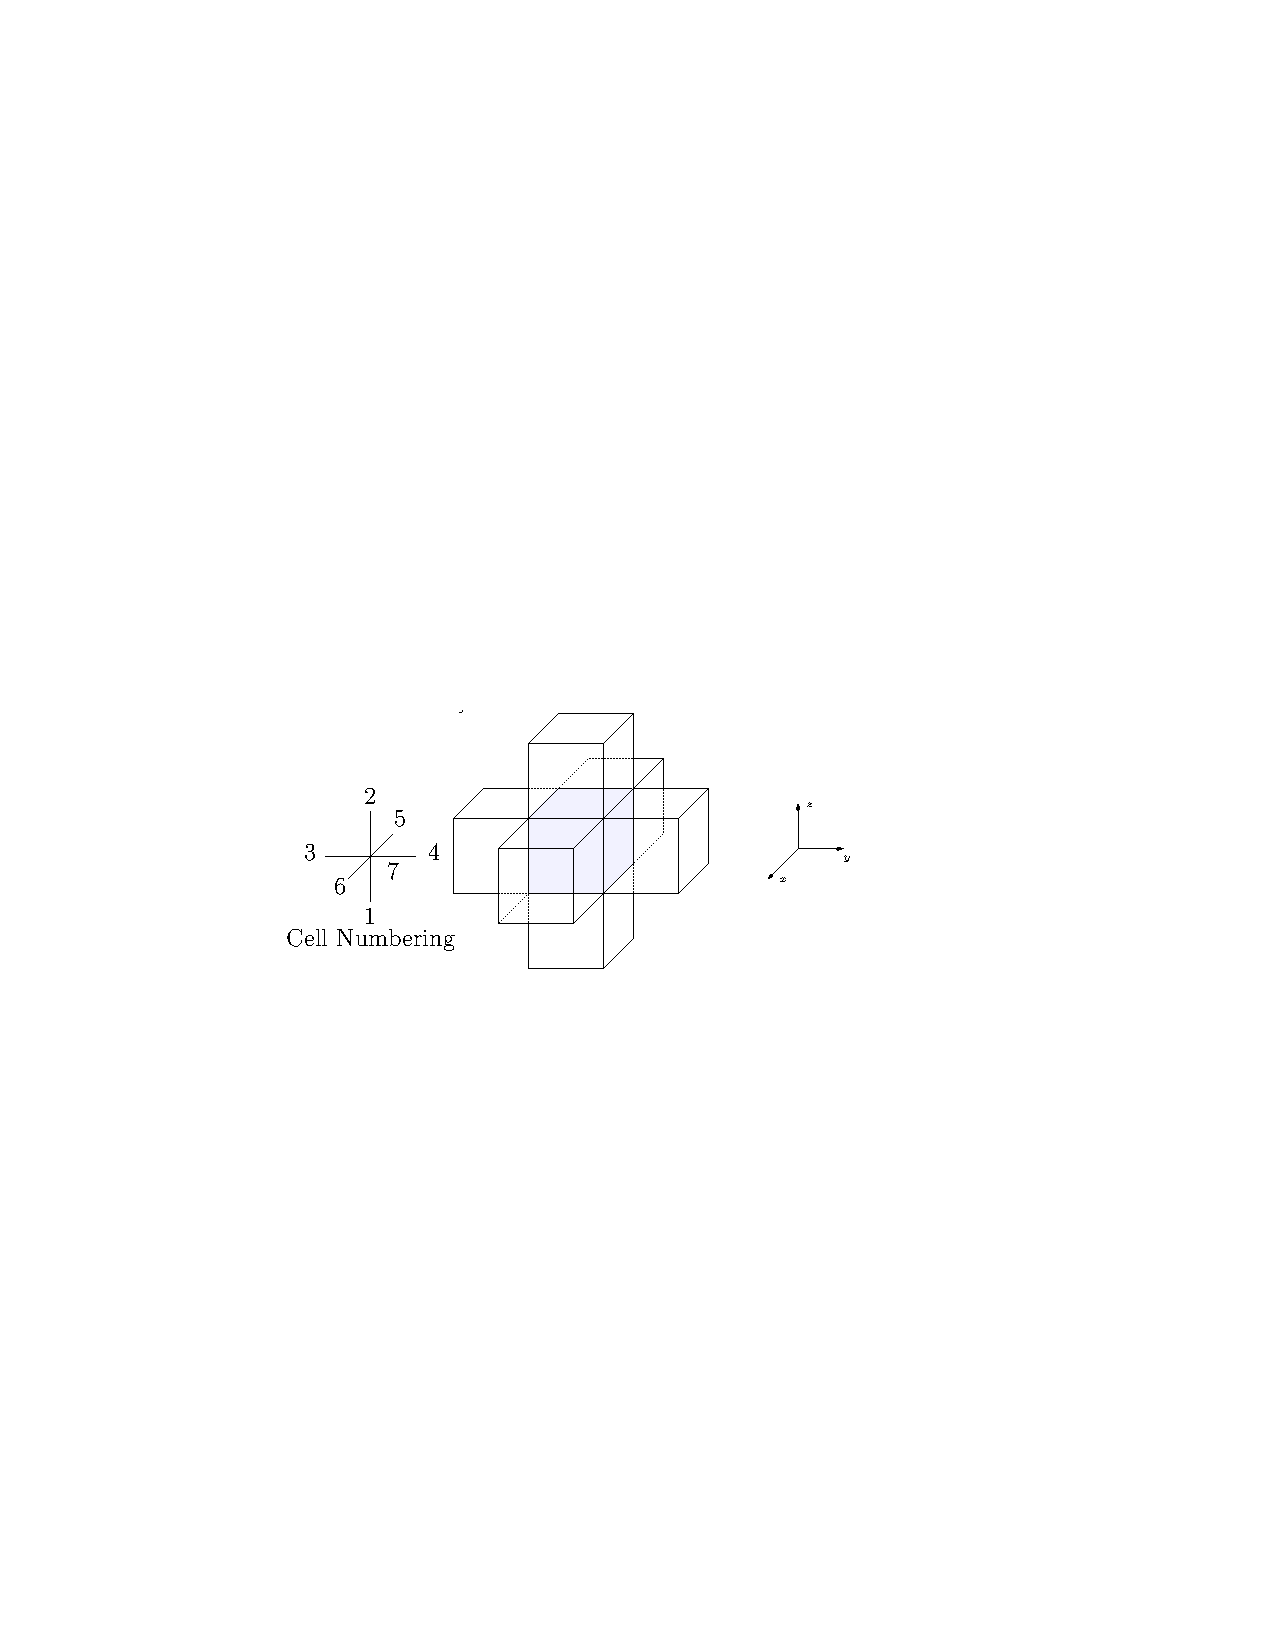
\includegraphics[clip]{3D_mesh_segment.pdf}}
  \caption{3D mesh-segment.  The particle's current cell (in blue) is
    connected to 6 adjacent cells.  The cell numbers are plotted
    alongside the mesh such that the blue cell has index 7, the high
    $z$ cell has index 2, etc.}
  \label{fig:mesh_segment}
\end{figure}

%%---------------------------------------------------------------------------%%
\section{Results}
\label{sec:results}

Here we examine the effectiveness of the MCSA method and compare it to
traditional deterministic solution methods.  The deterministic methods
considered are preconditioned Conjugate Gradient (PCG) and
preconditioned fixed-point (Richardson) iteration (PFIX).  The PCG
method uses right-left preconditioning with $\ve{M}=\ve{L}\ve{L}^{T}$,
where $\ve{L} = \ve{L}^{T} = \sqrt{\diag(\ve{D})}$.  Naturally, more
powerful preconditioning methods could be used; however, this provides
a fair comparison with the preconditioning used in the MCSA method.
Different preconditioning strategies within MCSA will be the focus of
a future paper.  The PFIX scheme is used to solve
Eq.~(\ref{eq:preconditioned-diffusion}), which is identical to the
system being solved with MCSA.  We examine each method on two 3D
problems: a Marshak wave problem and a multi-material duct problem.

\subsection{Marshak Wave}

The Marshak wave problem under consideration in this study has an incoming
1~keV blackbody boundary flux at $x=0$ and propagates in the $x$-dimension in
time as outlined in Ref.~\cite{larsen_1980}.  In other words, this is a 3D
representation of a 1D problem.  The full set of problem conditions is as
follows:
\begin{center}
  \begin{tabular}{ll}\hline
    B.C. & $f_b^{+}(x=0,T=1.0) = \frac{ac}{4}T^4$ \\ & $\ve{F} =
    0\quad \partial\Gamma \in \{x^{+}, y^{-}, y^{+}, z^{-}, z^{+}\}$
    \\ material properties & $\rho =
    3.0\,\text{g}\cdot\text{cm}^{-3}$ \\ & $\Cv =
    0.1\,\text{GJ}\cdot\text{g}^{-1}\cdot\text{keV}^{-1}$\\ &
    $T(t=0) = \sn{1}{-4}\,\text{keV}$\\  opacity & $\sigma =
    100T^{-3}\,\text{cm}^2\cdot\text{g}^{-1}$ \\  mesh & $\Di = \Dj
    = \Dk = 0.01\,\text{cm}$ \\ & $N_i = 100\quad N_j = N_k = 4$
    \\ \hline
  \end{tabular}
\end{center}
The problem is run to $100$~nanoseconds.

Figure~\ref{fig:marshak_10} shows the analytic Marshak Wave solution compared
to the MCSA solution.  As opposed to most Monte Carlo techniques, the MCSA
method generates solutions that are numerically equivalent to the PCG and PFIX
results.  Because the MCSA method converges the residual of the system, the
numerical accuracy is determined by the stopping criterion shown in
Eq.~(\ref{eq:stopping-criteria}).  Also, the MCSA method is not bound by the
Central Limit Theorem so convergence is not restricted to
$1/\sqrt{N}$~\cite{halton_1994,evans_2003}.
\begin{figure}[ht!]
  \centerline{ 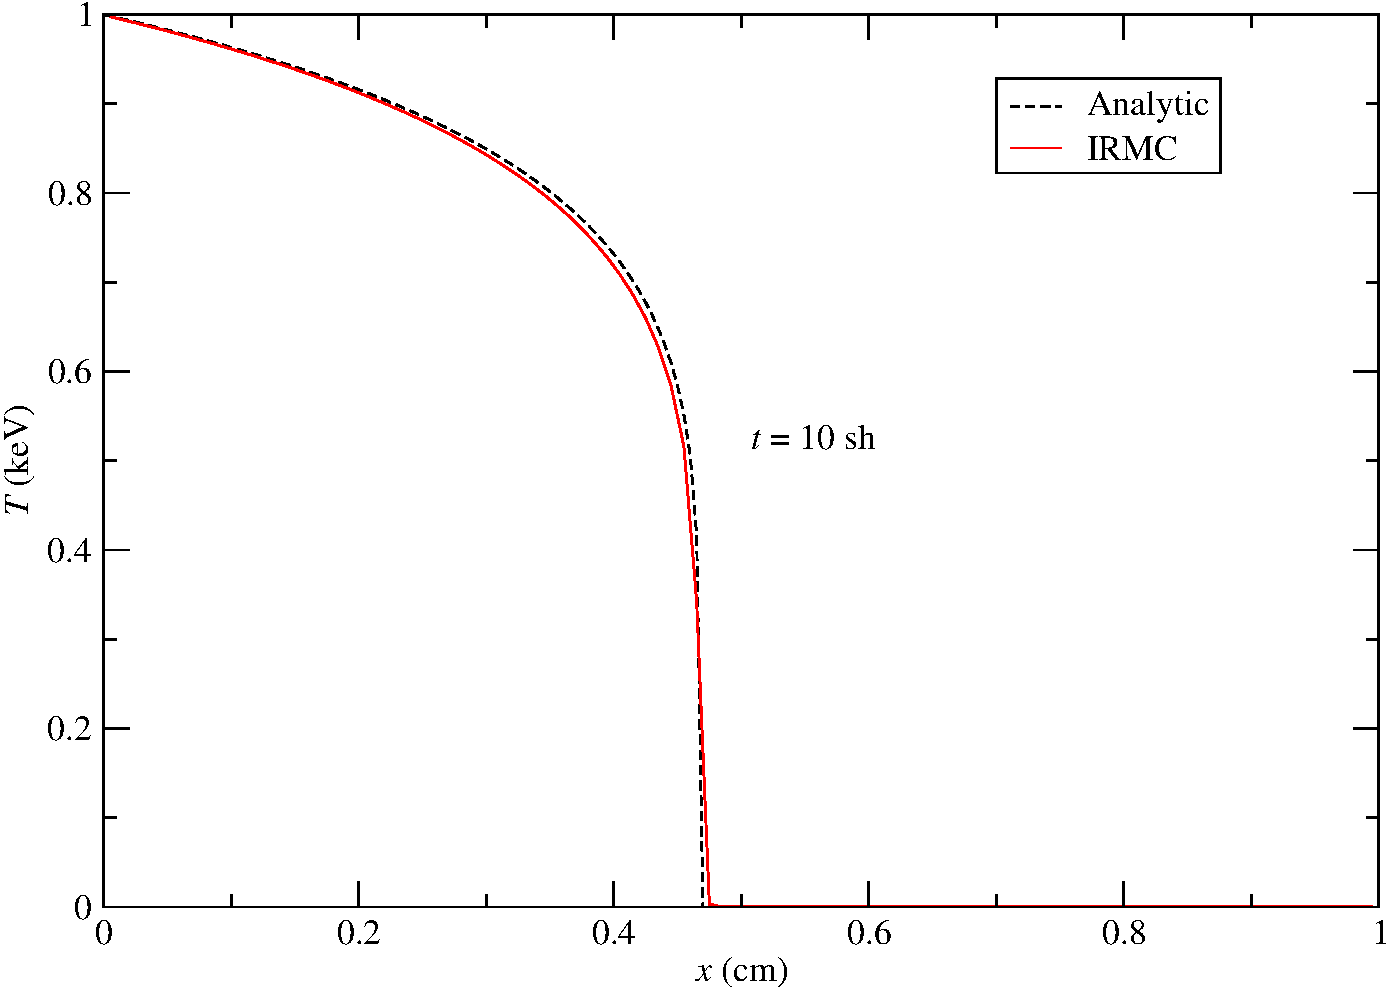
\includegraphics[width=5in,clip]{marshak_10.pdf}}
  \caption{ Solution of the Marshak wave problem at $t=100$~ns.  The analytic
    solution is compared to the MCSA solution.  The MCSA, PCG, and PFIXED
    methods are all converged to the same tolerance and therefore give
    numerically equivalent answers.}
  \label{fig:marshak_10}
\end{figure}

As stated in \S~\ref{sec:monte-carlo-matrix}, the MCSA method will converge
when $\rho(\ve{H})< 1$, where $\ve{H}$ is the iteration matrix and is defined
$\ve{H} = (\vI - \ve{M}^{-1}\ve{D})$.  The spectral radius for the Marshak
problem is plotted in Figure~\ref{fig:marshak_spectral}.  As described in
\S~\ref{sec:preconditioning}, the preconditioning effectively reduces the
spectral radius of $\ve{H}$ to less than 1.
\begin{figure}[ht!]
  \centerline{ 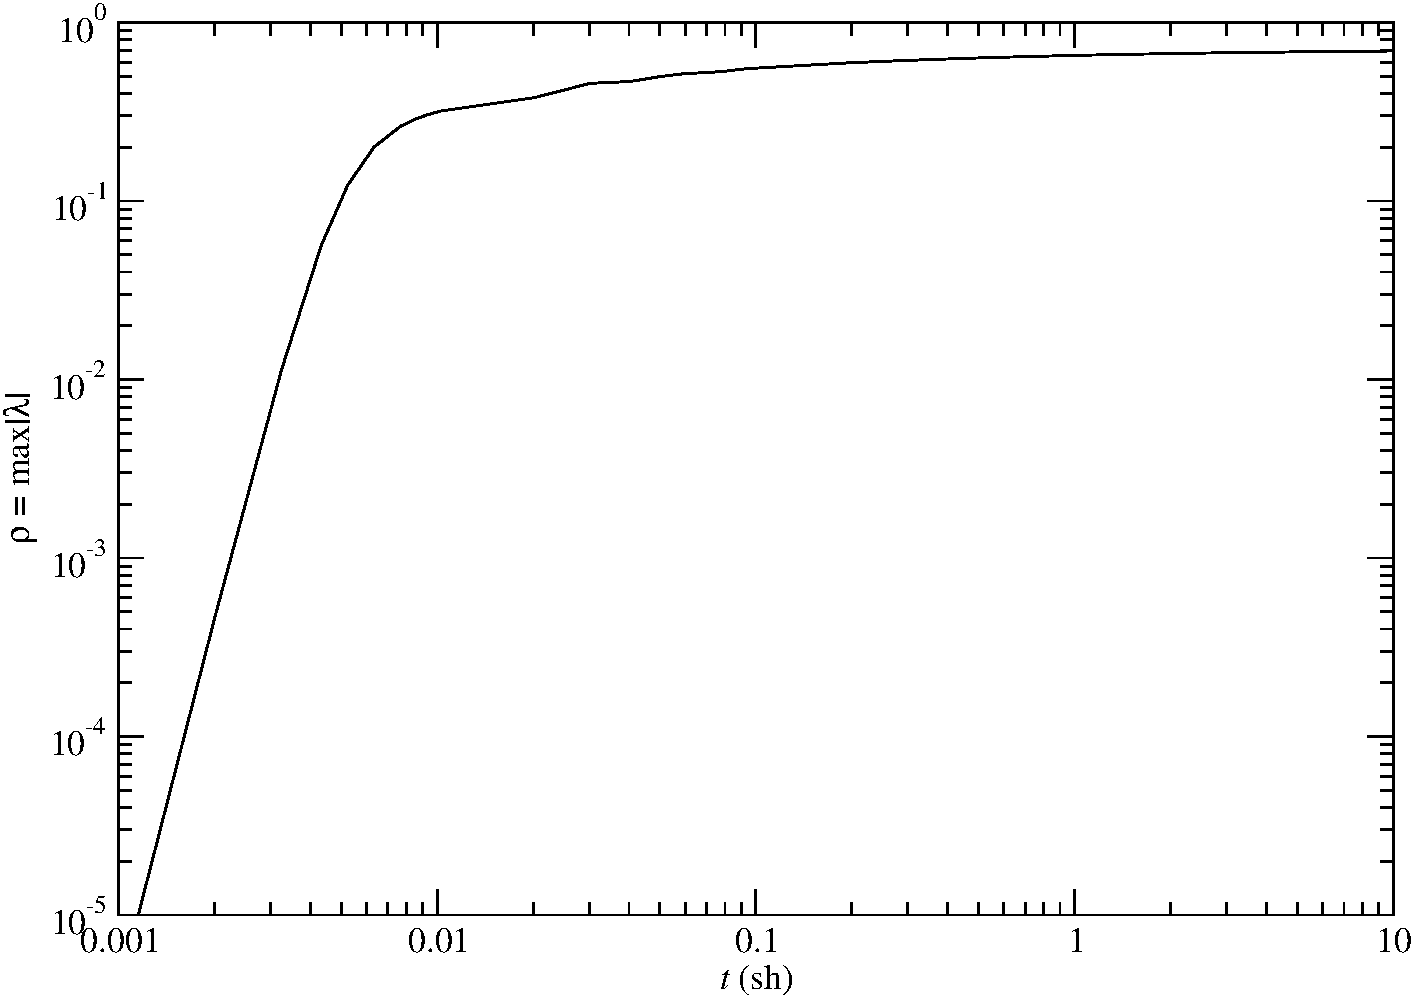
\includegraphics[width=5in,clip]{spectral_radius.pdf}}
  \caption{Spectral radius of the iteration matrix, $\ve{H}$, for the
    Marshak Wave problem as a function of elapsed problem time.}
  \label{fig:marshak_spectral}
\end{figure}

There are two principal degrees of freedom when utilizing the MCSA method: (1)
the number of particles per stage and (2) the weight cutoff.
Figure~\ref{fig:CPU_Np} shows the CPU time as a function of the requested
number of particles per stage for a relative weight cutoff of $\sn{1}{-4}$.
For less than five particles per stage, the method does not converge.
Figure~\ref{fig:CPU_Ns} shows the variation in the maximum number of stages
(iterations) per cycle with number of particles.  Analysis of these two
figures shows that increasing the number of particles per stage reduces the
number of iterations required to converge the solution.  However, the cost of
the Monte Carlo transport is high; thus, better performance is attained by
running more stages with fewer particles per stage \cite{evans_2003}.
\begin{figure}[ht!]
  \centerline{ 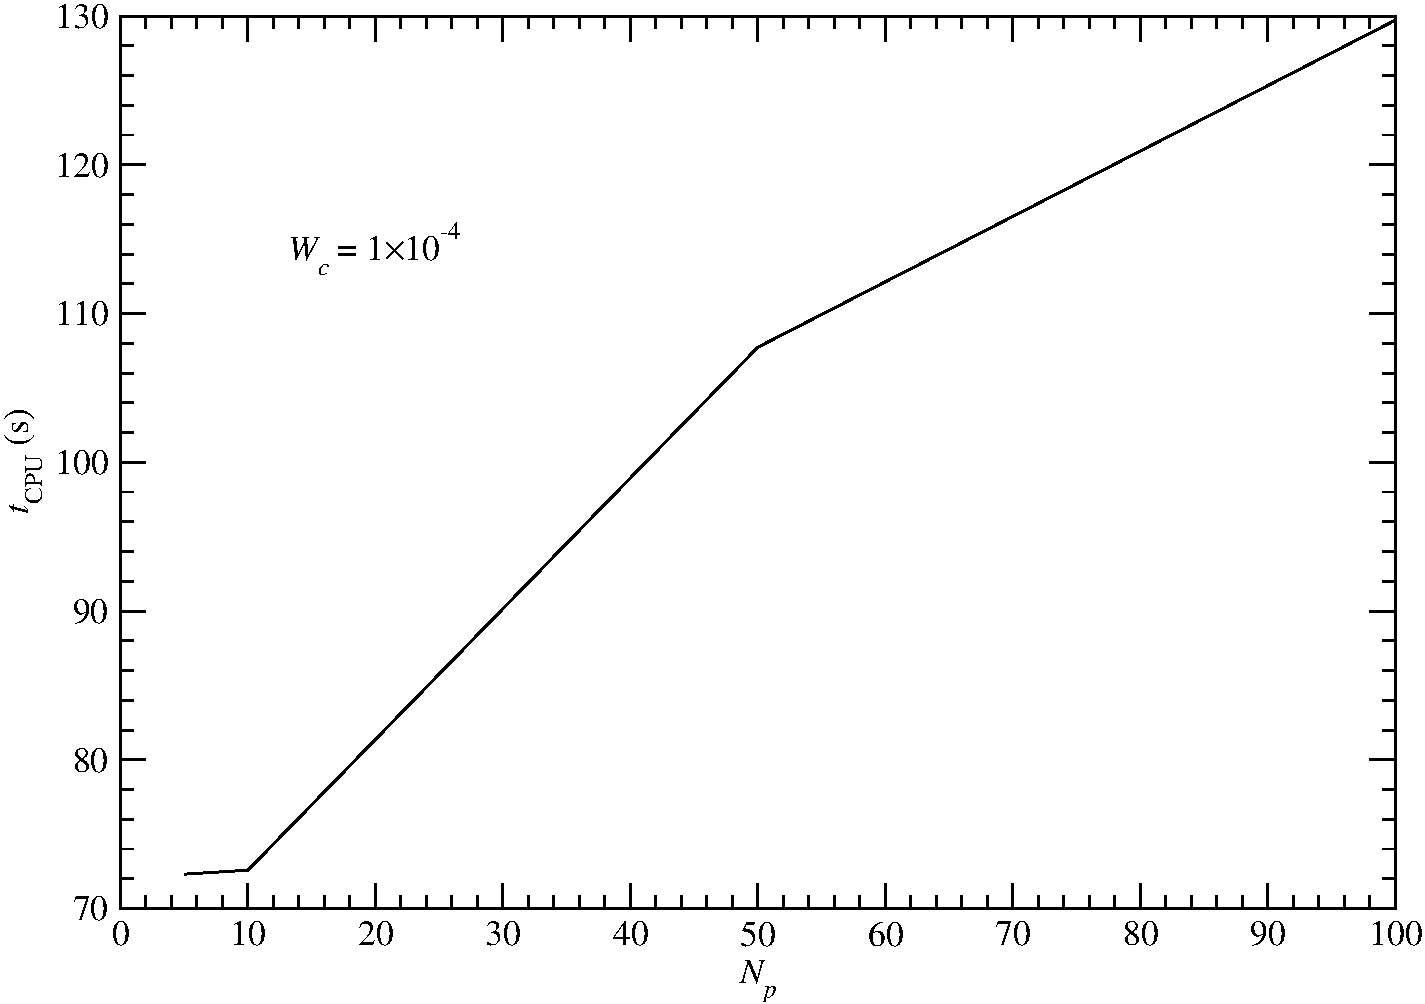
\includegraphics[width=5in,clip]{mrshk_np_CPU.pdf}}
  \caption{CPU time versus number of particles per stage for the
    Marshak problem.  The number of particles is the requested number.
    In each stage the exact number can vary depending upon the number
    of cells and source strength per cell.}
  \label{fig:CPU_Np}
\end{figure}

\begin{figure}[ht!]
  \centerline{ 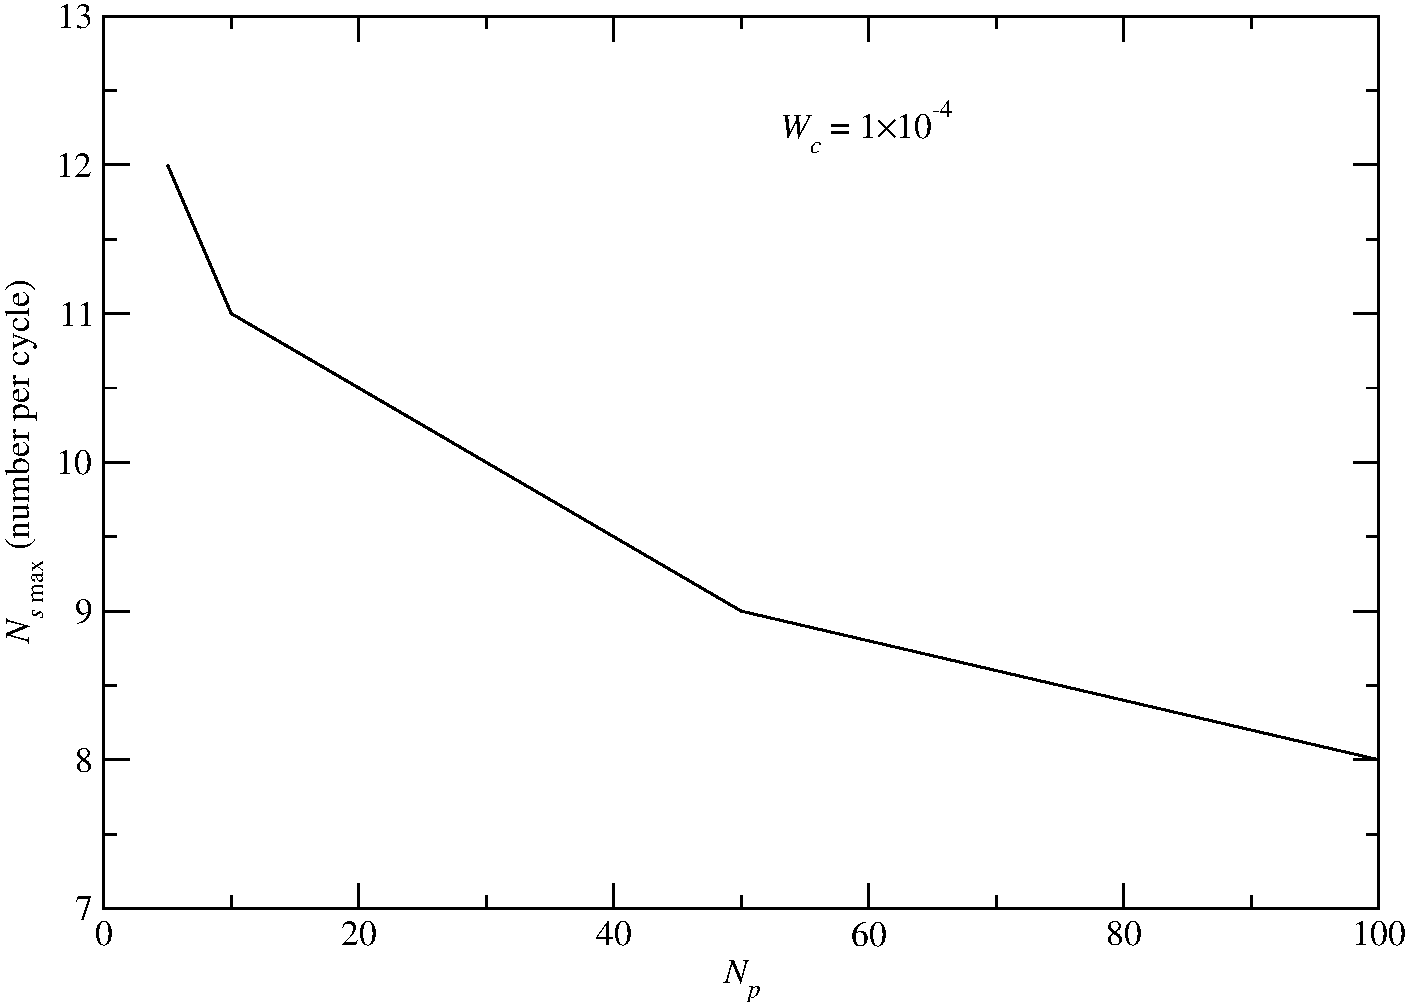
\includegraphics[width=5in,clip]{mrshk_np_Ns.pdf}}
  \caption{ Maximum number of stages per cycle versus number of
    particles per stage for the Marshak problem.  The number of
    particles is the requested number.  In each stage the exact number
    can vary depending upon the number of cells and source strength
    per cell.}
  \label{fig:CPU_Ns}
\end{figure}

Figure~\ref{fig:CPU_wc} shows the CPU time as a function of relative weight
cutoff.  These results indicate that the performance of the MCSA method is
relatively insensitive to the weight cutoff.  This is especially true when
running small numbers of particles per stage.  The weight cutoff has a more
pronounced effect on the efficiency of the method when larger numbers of
particles are used.
\begin{figure}[ht!]
  \centerline{ 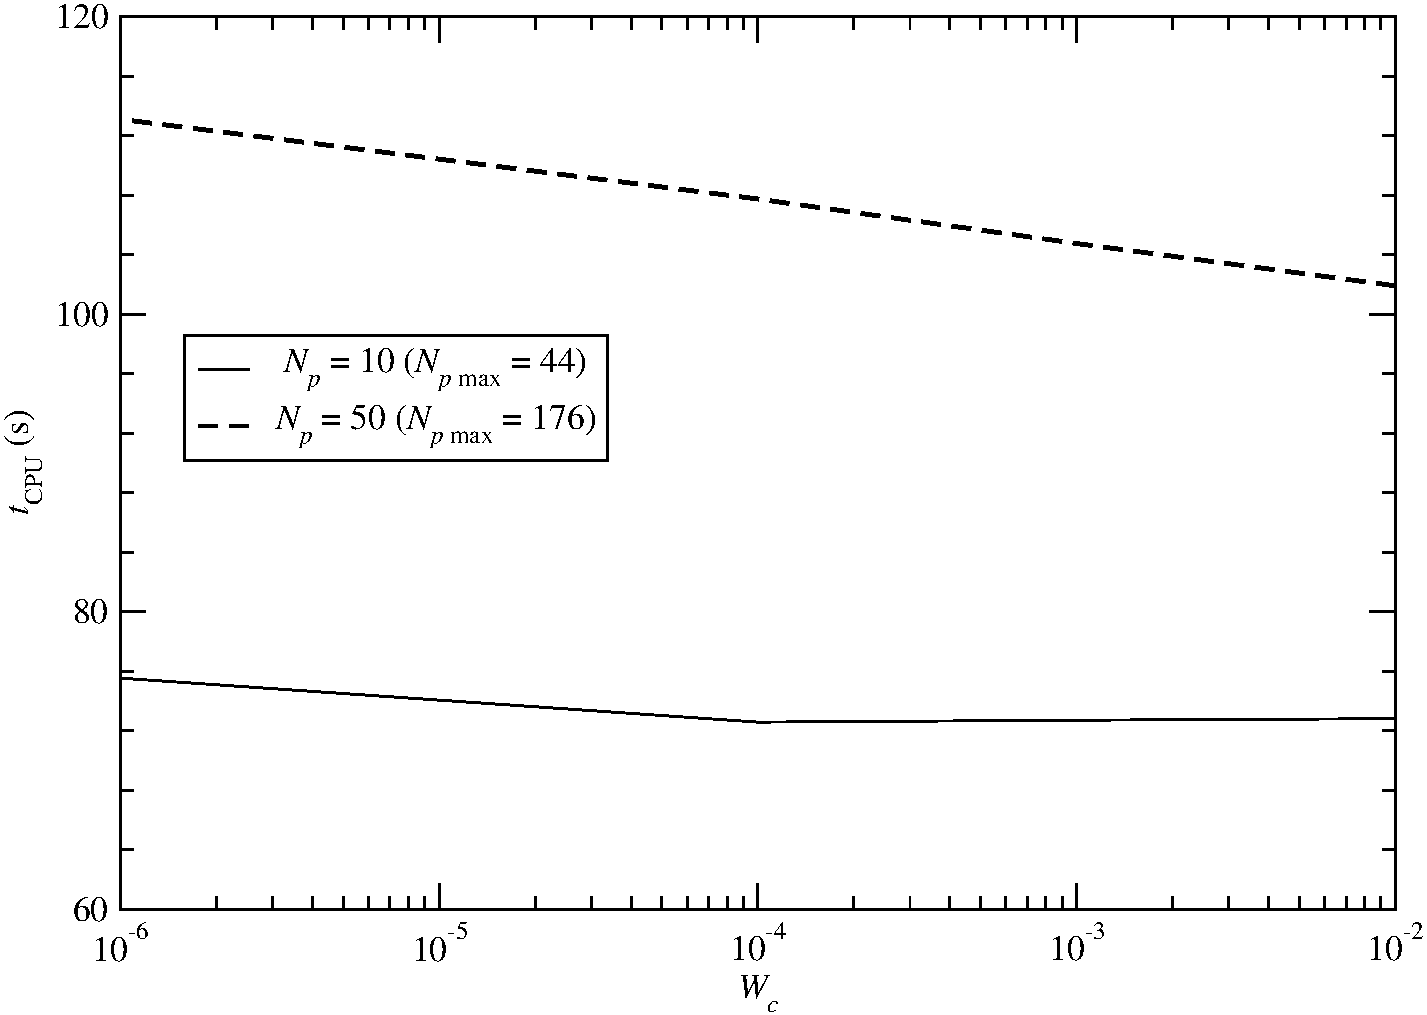
\includegraphics[width=5in,clip]{mrshk_wc_CPU.pdf}}
  \caption{ CPU time versus relative weight cutoff for the Marshak
    problem.  Results are shown for 10 and 50 requested particles per
    stage.  The numbers in parentheses show the maximum number of
    particles run in a stage during the course of the problem.}
  \label{fig:CPU_wc}
\end{figure}

Having analyzed the variation of the MCSA algorithm efficiency with number of
particles and weight cutoff, we now compare to traditional deterministic
algorithms.  Table~\ref{tab:marshak_comparison} shows timing results for the
Marshak problem using preconditioned CG (PCG), preconditioned Richardson
iteration (PFIX), and MCSA. The results show that the MCSA method is the most
efficient method, although the PCG results are nearly as fast.  More
importantly, the MCSA method clearly accelerates Richardson iteration, as
indicated by the fact that MCSA is 42\% faster than Richardson iteration
alone.
\begin{table}[ht!]
  \caption{Comparison of solution methods for the Marshak problem. All
    methods were run with a stopping criterion of $\sn{1}{-8}$.  The
    MCSA method used $N_p=10$ and $W_c = \sn{1}{-4}$.  The CPU time is
    measured relative to the MCSA method, which required 72.6 s on a
    3.6~GHz Xeon.}
  \label{tab:marshak_comparison}
  \begin{center}
    \begin{tabular}{lrr}\hline\hline
      \multicolumn{1}{c}{Method} & \multicolumn{1}{c}{Max Iterations}
      & \multicolumn{1}{c}{Relative CPU Time}\\\hline\hline  PCG &
      11 & 1.11 \\  PFIX & 11 & 1.42 \\  MCSA & 11 & 1.0
      \\ \hline\hline
    \end{tabular}
  \end{center}
\end{table}

\subsection{Multi-material Problem}

We now test the performance of the MCSA method on a large multi-material
problem.  The multi-material problem has a dog-legged duct through a thick
wall where the radiation flows into a thin region bound by a foil on one side.
The mesh and geometry are illustrated in Figure~\ref{fig:multi-mat-mesh}.  A
blackbody boundary flux is defined on the low-$x$ face at $T=0.5$~keV.  The
full set of problem conditions is as follows:
\begin{center}
  \begin{tabular}{ll}\hline
    B.C. & $f_b^{+}(x=0,T=0.5) = \frac{ac}{4}T^4$\\ & $\ve{F} =
    0\quad \partial\Gamma \in \{x^{+}, y^{-}, y^{+}, z^{-}, z^{+}\}$
    \\  material properties & $\rho =
    1.5\,\text{g}\cdot\text{cm}^{-3}$ (duct) \\ & $\rho =
    8.0\,\text{g}\cdot\text{cm}^{-3}$ (wall) \\ & $\rho =
    4.0\,\text{g}\cdot\text{cm}^{-3}$ (foil) \\ & $\Cv =
    0.1\,\text{GJ}\cdot\text{g}^{-1}\cdot\text{keV}^{-1}$\\ &
    $T(t=0) = \sn{1}{-4}\,\text{keV}$\\  opacity & $\sigma =
    T^{-3}\,\text{cm}^2\cdot\text{g}^{-1}$ (duct) \\ & $\sigma =
    1000T^{-1}\,\text{cm}^2\cdot\text{g}^{-1}$ (wall) \\ & $\sigma =
    5T^{-2}\,\text{cm}^2\cdot\text{g}^{-1}$ (foil) \\  mesh & $\Di =
    \Dj = \Dk = 0.025\,\text{cm}$ \\ & $N_i = N_j = N_k = 60$
    \\ \hline
  \end{tabular}
\end{center}

A 2D plot of the temperature at 1000~ns elapsed time is illustrated in
Figure~\ref{fig:multi-mat_T}.  The time evolution of the temperature is shown at
four edit points in Figure~\ref{fig:edit-points}.  All three methods, PCG, PFIX,
and MCSA, give numerically identical answers when using a stopping criterion
of $\sn{1}{-8}$.
\begin{figure}[ht!]
  \centerline{ 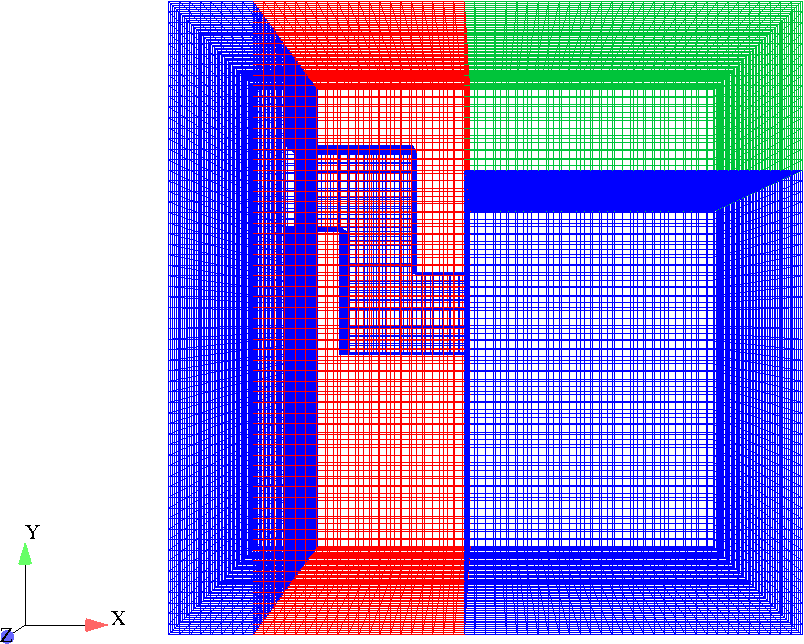
\includegraphics[width=5in,clip]{mesh.pdf}}
  \caption{Multi-material problem mesh.  The duct region is blue.  The wall is
    red.  The foil is green.  The mesh is $60\times 60\times 60$.}
  \label{fig:multi-mat-mesh}
\end{figure}

\begin{figure}[ht!]
  \centerline{ 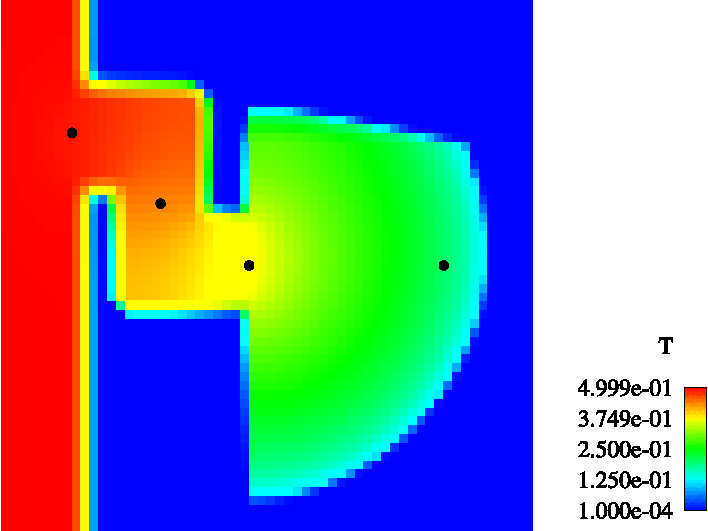
\includegraphics[width=5in,clip]{T_multi_mat.pdf}}
  \caption{ Two-dimensional plot of the temperature in keV at 1000~ns
    on a cut-plane positioned at the mid-point of the $z$-axis.  The
    positions of the edit points where the time evolution of the
    temperature is plotted in Figure~\ref{fig:edit-points} are
    indicated by the black disks.}
  \label{fig:multi-mat_T}
\end{figure}

\begin{figure}[ht!]
  \begin{center}
    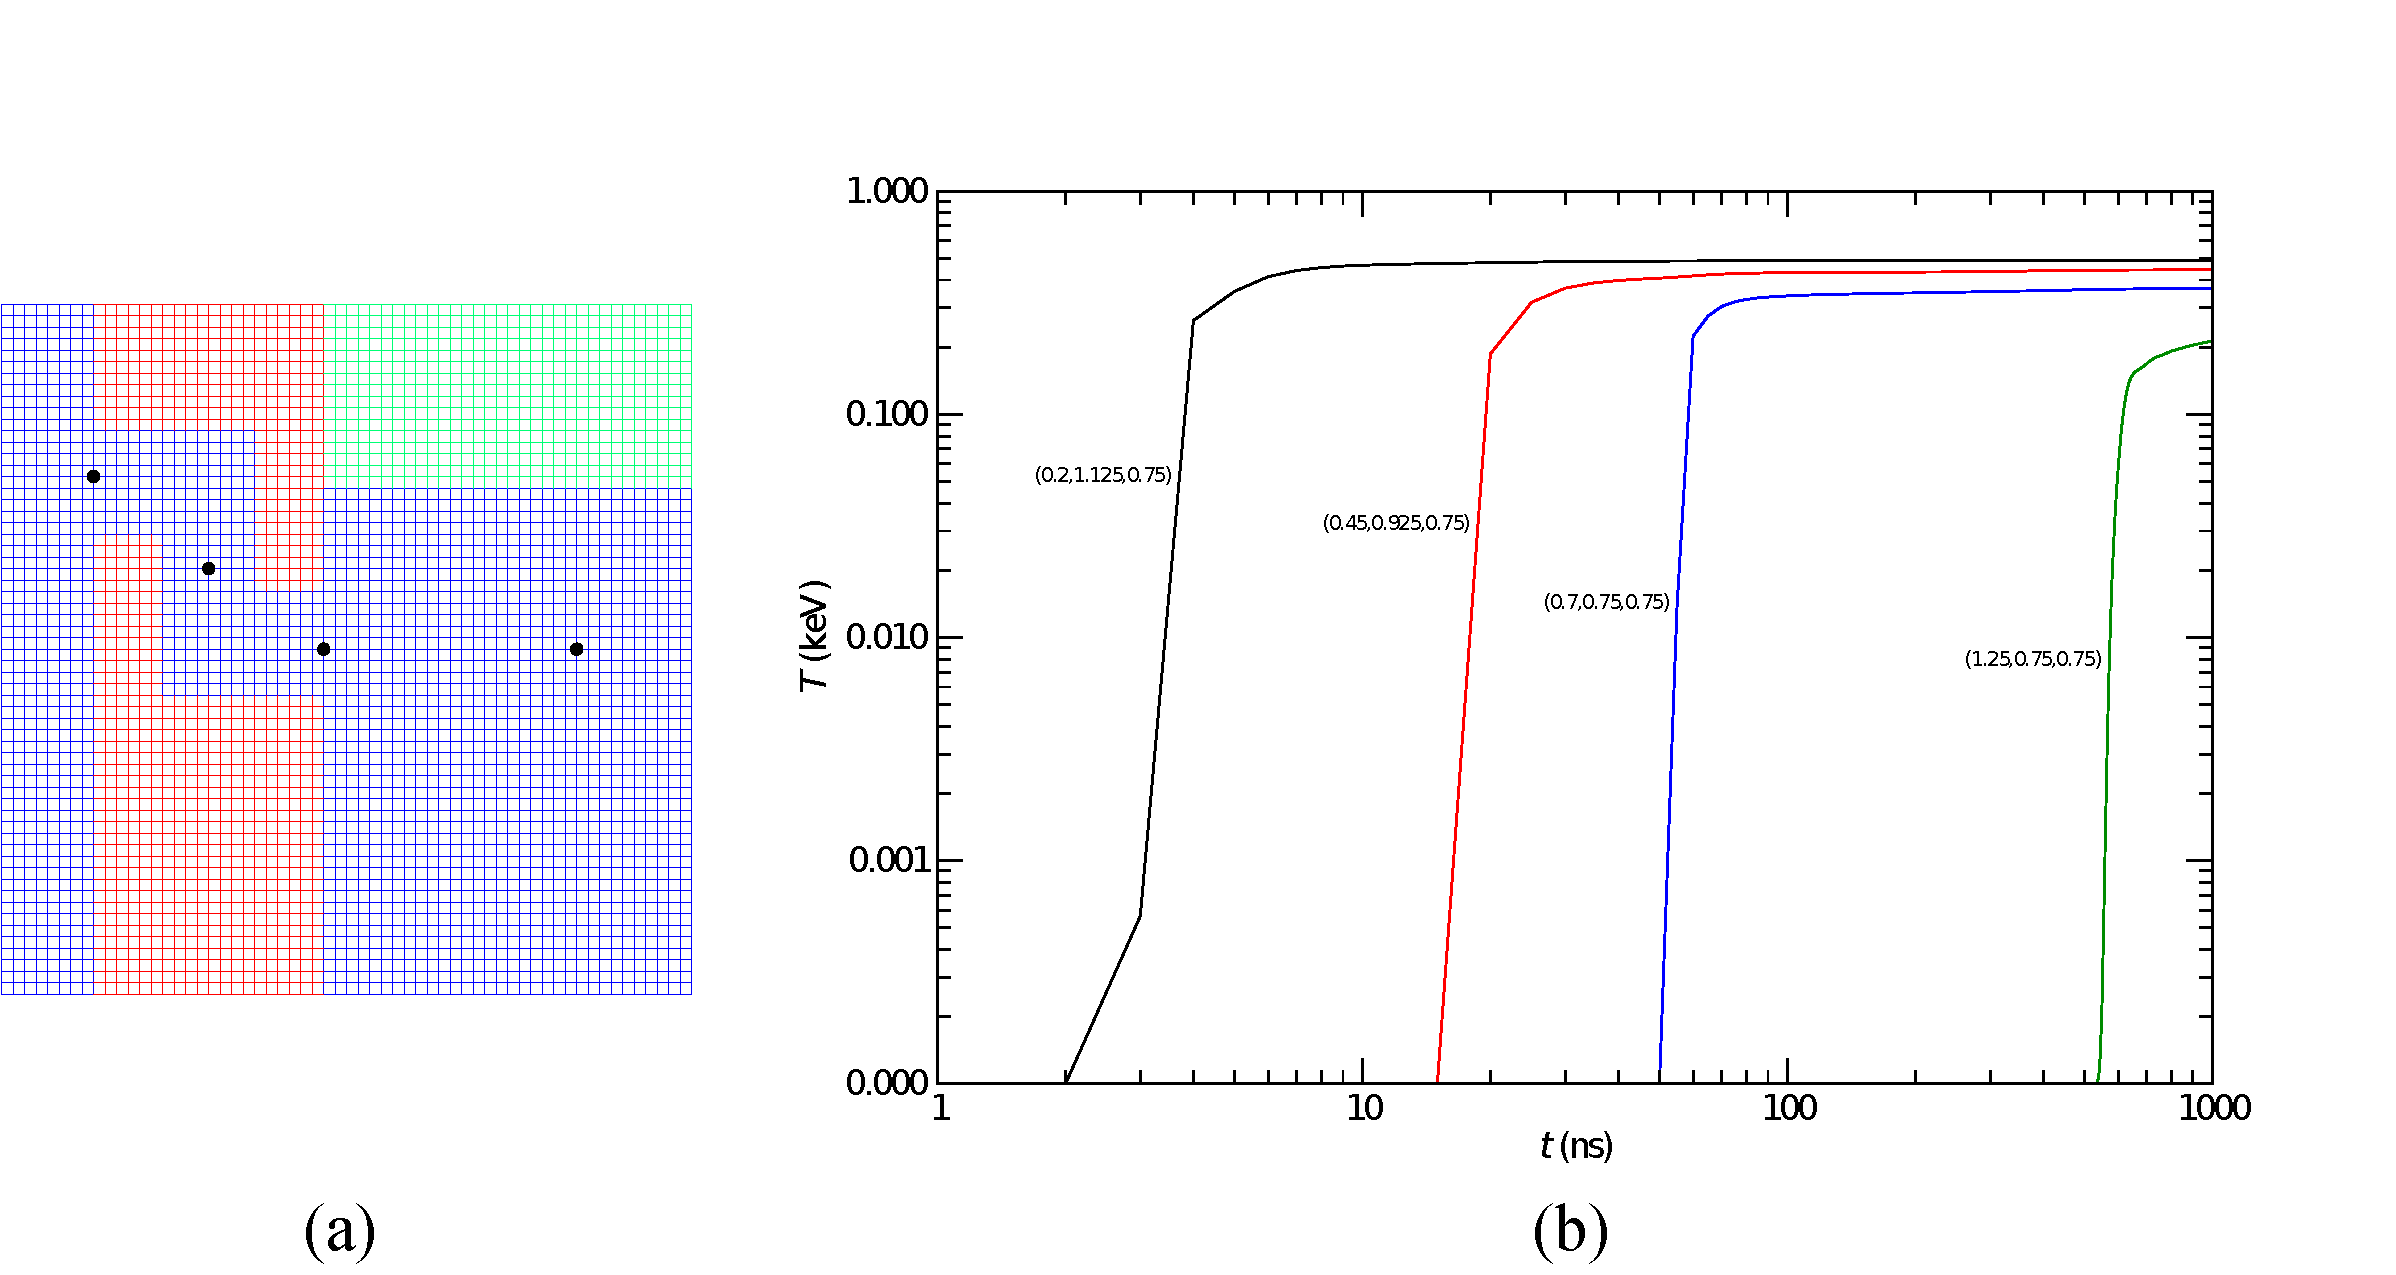
\includegraphics[width=5in,clip]{edit_points.pdf}
  \end{center}
  \caption{(a) Edit points and (b) time-evolution of the temperature at each
    point.  All points are centered in the $z$-axis.}
  \label{fig:edit-points}
\end{figure}

Table~\ref{tab:multimat_comparison} shows the timing results for the
multi-material problem using PCG, PFIX, and MCSA.  The results correspond
roughly with the results from the Marshak problem.  The MCSA is marginally
faster than PCG and 43\% faster than PFIX.
\begin{table}[htbp!]
  \caption{ Comparison of solution methods for the multi-material
    problem. All methods were run with a stopping criterion of
    $\sn{1}{-8}$.  The MCSA method used $N_p=1000$ and $W_c =
    \sn{1}{-3}$.  The problem was run to an elapsed time of 100~ns.
    The MCSA method required 3.4 hours on a 3.6~GHz Xeon.}
  \label{tab:multimat_comparison}
  \begin{center}
    \begin{tabular}{lrr}\hline\hline
      \multicolumn{1}{c}{Method} & \multicolumn{1}{c}{Max Iterations}
      & \multicolumn{1}{c}{Relative CPU Time}\\\hline\hline  PCG &
      18 & 1.03 \\  PFIX & 38 & 1.43 \\  MCSA & 20 & 1.0
      \\ \hline\hline
    \end{tabular}
  \end{center}
\end{table}

%%---------------------------------------------------------------------------%%
\section{Conclusions}
\label{sec:conclusions}

We have presented a new Monte Carlo solution method for solving the discrete,
time-dependent radiation diffusion equation in three dimensions.  The MCSA
method has been shown to match results using standard solution techniques to
arbitrary precision. Also, the new method has been to shown to be faster than
preconditioned CG and Richardson iteration for the model problems presented
here.

While we have demonstrated marginal improvements over standard solution
schemes in this study, significant improvements could be realized in fully
nonlinear-consistent solutions.  In these cases, the MCSA method competes with
GMRES, which is more costly in memory and time than CG.  Another area where
the MCSA scheme may have advantages over traditional solution methods is on
dentritic, or adaptive, meshes.  These meshes yield matrices with poor
condition numbers because of the changing cell volumes at different refinement
levels.  A smart transport algorithm could be developed that more efficiently
solves the residual on these types of meshes.  These topics will be the focus
of future study.

%%---------------------------------------------------------------------------%%
\section*{Acknowledgements}

Work for this paper was supported by Oak Ridge National Laboratory, which is
managed and operated by UT-Batelle, LLC, for the U.S. Department of Energy under
Contract No. DEAC05-00OR22725.

%%---------------------------------------------------------------------------%%
%% The Appendices part is started with the command \appendix;
%% appendix sections are then done as normal sections
%% \appendix

%% \section{}
%% \label{}

%% References
%%
%% Following citation commands can be used in the body text:
%% Usage of \cite is as follows:
%%   \cite{key}         ==>>  [#]
%%   \cite[chap. 2]{key} ==>> [#, chap. 2]
%%

%%---------------------------------------------------------------------------%%
%% References with bibTeX database:

\bibliographystyle{elsarticle-num} 
\bibliography{references}

%% Authors are advised to submit their bibtex database files. They are
%% requested to list a bibtex style file in the manuscript if they do
%% not want to use elsarticle-num.bst.

%% References without bibTeX database:

% \begin{thebibliography}{00}

%% \bibitem must have the following form:
%%   \bibitem{key}...
%%

% \bibitem{}

% \end{thebibliography}

%%---------------------------------------------------------------------------%%

\end{document}

%%
%% End of file `jcomp2012.tex'.
